% Options for packages loaded elsewhere
\PassOptionsToPackage{unicode}{hyperref}
\PassOptionsToPackage{hyphens}{url}
%
\documentclass[
]{article}
\usepackage{lmodern}
\usepackage{amssymb,amsmath}
\usepackage{ifxetex,ifluatex}
\ifnum 0\ifxetex 1\fi\ifluatex 1\fi=0 % if pdftex
  \usepackage[T1]{fontenc}
  \usepackage[utf8]{inputenc}
  \usepackage{textcomp} % provide euro and other symbols
\else % if luatex or xetex
  \usepackage{unicode-math}
  \defaultfontfeatures{Scale=MatchLowercase}
  \defaultfontfeatures[\rmfamily]{Ligatures=TeX,Scale=1}
\fi
% Use upquote if available, for straight quotes in verbatim environments
\IfFileExists{upquote.sty}{\usepackage{upquote}}{}
\IfFileExists{microtype.sty}{% use microtype if available
  \usepackage[]{microtype}
  \UseMicrotypeSet[protrusion]{basicmath} % disable protrusion for tt fonts
}{}
\makeatletter
\@ifundefined{KOMAClassName}{% if non-KOMA class
  \IfFileExists{parskip.sty}{%
    \usepackage{parskip}
  }{% else
    \setlength{\parindent}{0pt}
    \setlength{\parskip}{6pt plus 2pt minus 1pt}}
}{% if KOMA class
  \KOMAoptions{parskip=half}}
\makeatother
\usepackage{xcolor}
\IfFileExists{xurl.sty}{\usepackage{xurl}}{} % add URL line breaks if available
\IfFileExists{bookmark.sty}{\usepackage{bookmark}}{\usepackage{hyperref}}
\hypersetup{
  pdftitle={Relationship between Spread of COVID-19 and Race and Ethnicity Demographics},
  pdfauthor={Jordan Meyer, Justin Peabody, Aswin Thiruvengadam, Leon Gutierrez},
  hidelinks,
  pdfcreator={LaTeX via pandoc}}
\urlstyle{same} % disable monospaced font for URLs
\usepackage[margin=1in]{geometry}
\usepackage{graphicx,grffile}
\makeatletter
\def\maxwidth{\ifdim\Gin@nat@width>\linewidth\linewidth\else\Gin@nat@width\fi}
\def\maxheight{\ifdim\Gin@nat@height>\textheight\textheight\else\Gin@nat@height\fi}
\makeatother
% Scale images if necessary, so that they will not overflow the page
% margins by default, and it is still possible to overwrite the defaults
% using explicit options in \includegraphics[width, height, ...]{}
\setkeys{Gin}{width=\maxwidth,height=\maxheight,keepaspectratio}
% Set default figure placement to htbp
\makeatletter
\def\fps@figure{htbp}
\makeatother
\setlength{\emergencystretch}{3em} % prevent overfull lines
\providecommand{\tightlist}{%
  \setlength{\itemsep}{0pt}\setlength{\parskip}{0pt}}
\setcounter{secnumdepth}{5}
\usepackage{rotating, graphicx, geometry}
\usepackage{rotating}
\usepackage{booktabs}
\usepackage{longtable}
\usepackage{array}
\usepackage{multirow}
\usepackage{wrapfig}
\usepackage{float}
\usepackage{colortbl}
\usepackage{pdflscape}
\usepackage{tabu}
\usepackage{threeparttable}
\usepackage{threeparttablex}
\usepackage[normalem]{ulem}
\usepackage{makecell}
\usepackage{xcolor}

\title{Relationship between Spread of COVID-19 and Race and Ethnicity
Demographics}
\author{Jordan Meyer, Justin Peabody, Aswin Thiruvengadam, Leon Gutierrez}
\date{04/14/21}

\begin{document}
\maketitle

{
\setcounter{tocdepth}{2}
\tableofcontents
}
\newpage

\newpage
\setlength{\headsep}{1cm}
\maketitle

\newpage
\setlength{\headsep}{1cm}

\section{Introduction}

The rapid global spread of Coronavirus-19(SARS-Cov-2) caught households
and governments by surprise. Yet, based on history, pandemic researchers
have been warning about the likelihood of such an event. So far this
century, the world has already confronted an array of viral scares,
Severe Acute Respiratory Syndrome (SARS), H1N1(Swine flu), Middle East
respiratory syndrome (MERS), Ebola, Zika and Dengue. This increase has
been attributed to urbanization, globalization and increased human
consumption of animal proteins as society becomes more
prosperous\textsuperscript{{[}1{]}}

Touted as the ``great equalizer'' that transcends wealth, fame, prestige
and age\textsuperscript{{[}2{]}}, in reality, Coronavirus-19 has had a
varied impact on different social, economic, racial and ethinic
demographics\textsuperscript{{[}3{]}}. In this research, we focus on
race and ethnicity demographics. A report from the Center for Disease
Control and Prevention (hereafter referred to as the CDC)
observed\textsuperscript{{[}3{]}} that People of Color (POC) are much
more likely to get infected, hospitalized and die from Coronavirus-19
and hence in this research question we analyze the relationship of
Coronavirus-19 cases between people of different ethnicities.
Specifically, our research question is:

\textbf{\emph{Is a higher percentage of People of Color, or Hispanic or
Latino population associated with an increased incidence of
Coronavirus-19 cases per hundred thousand residents, in the conterminous
United States?}}

People of Color in the scope of this research are defined as people who
do not identify as belonging to a white race only. Hispanic or Latino as
a demographic is an ethnicity and not a race, i.e.~a person of Latin
origin could identify as white or any other race. Hence we include both
as separate variables.

The primary COVID data source provided as part of this study are state
level statistics of Coronavirus-19 cases and Coronavirus-19 death rates.
We consider two states to be equally affected by Coronavirus-19 only if
they have the same rate of occurrence of Coronavirus-19, i.e the number
of Coronavirus-19 cases as a fraction of the total populations is the
same. We chose the primary response variable as `cases per one hundred
thousand residents' for this reason. We consider two states to have
equal representation of people of color only if the rate of occurrence
of people of color is the same in the two states. Specifically, the
number of people of color as a fraction of the total population of the
state is the same between the two states. Hence we chose the
\emph{percentage of people of color in state population} as one of our
primary response variable. Similarly, we consider two states to have
equal representation of people who identify as Hispanic or Latino if the
rate of occurrence of people who identify as Hispanic or Latino is the
same in the two states. Specifically, the number of people who identify
as Hispanic or Latino as a fraction of the total population of the state
is the same between the two states.Hence we chose the \emph{percentage
of people who identify as Hispanic or Latino in state population} as one
of our primary response variable.

\newpage

\hypertarget{model-building-process}{%
\section{Model Building Process}\label{model-building-process}}

\hypertarget{objective-and-definitions}{%
\subsection{Objective and definitions}\label{objective-and-definitions}}

The overarching objective of our study is to answer the research
question in the context of covariate categories such as each state's
COVID policies(example: Stay at home mandates), each state's
socio-economic conditions(such as people below poverty line) and as
COVID spreads through physical proximity, each state's measured mobility
of people during the COVID time period of study.

\textbf{Definitions and terminology}

\begin{enumerate}
\def\labelenumi{\arabic{enumi}.}
\tightlist
\item
  Conterminous United States (hereafter referred to as CONUS) refers to
  the contiguous 48 states and includes Washington D.C. In the rest of
  this document we will use the short form CONUS instead.
\item
  In this document we will use the terms COVID-19 or COVID
  interchangeably with Coronavirus-19.
\item
  In the description of the datasets we will use \textbf{record} to
  describe the row of the table. Each record may contain values for
  several fields, these fields are the columns of the table. The term
  columns and fields will be used interchangeably in this document. The
  data engineering and the subsequent modeling of this data has been in
  the `R' programming language.
\item
  To reduce the confounding effects of the distribution of vaccines to
  the number of COVID cases, we have restricted the analysis to before
  the availability of vaccines in the United States. The first vaccine,
  outside the vaccine study, was administered on Dec 14th 2020. There
  are references to this date in the following sections we refer to it
  as the \emph{vaccine availability date}.
\item
  Mobility in the context of this study is the duration of time people
  spend at a given category of locations, such as parks or at their
  workplace, as compared to a baseline. These categories of parameters
  and their operationalizaiton will be discussed in detail in the
  following sections.
\item
  We also use the phrase \emph{time period of interest}. This denotes
  the time between 02/15/20 and the \emph{vaccine availability date}.
  02/15/20 is the date for the first record of the Google community
  mobility dataset described in detail in section 2.3.3
\end{enumerate}

\hypertarget{data-loading-and-cleaning}{%
\subsection{Data loading and cleaning}\label{data-loading-and-cleaning}}

We now provide the data sources we used for the analysis and a
description of their usage. We follow a consistent methodology in this
section:

\begin{enumerate}
\def\labelenumi{\arabic{enumi}.}
\tightlist
\item
  We provide a brief description of the raw data to provide the user
  context of its usage
\item
  We point to the section in the appendix which describes the process of
  obtaining this raw data
\item
  Also in the appendix is a description of converting the raw data into
  a processed table that is used for this analysis. Of the four datasets
  that were used for this analysis only one required this intermediate
  step
\item
  A description of the processed CSV
\item
  Steps of processing the CSV into operationalized variables for model
  generation. This section also contains the handling of missing data
\end{enumerate}

As we describe the above process, we also makes notes of any limitations
in the data which we later discuss in the `limitations of the model'
section(section 4)

\newpage

\subsection{Data description and processing individual datasets}

\hypertarget{new-york-times-covid-dataset}{%
\subsubsection{New York Times COVID
dataset}\label{new-york-times-covid-dataset}}

\textbf{``Data from The New York Times, based on reports from state and
local health agencies.'' }\\
\textbf{Hyperlink:
\href{https://github.com/nytimes/covid-19-data}{Github}}\\
\textbf{Data downloaded on: 03/25/2021 }

\hypertarget{summary-of-raw-data}{%
\paragraph{\texorpdfstring{Summary of raw data\\
}{Summary of raw data }}\label{summary-of-raw-data}}

New York Times has compiled an easily accessible dataset tracking daily
COVID cases and COVID related deaths for each state. The dataset is in
the format of a table where each row has five fields, namely, name of
the state, code for the state, date, number of COVID cases, number of
COVID deaths. The COVID cases on a given record (row) is the
\textbf{cumulative count} of all cases till that date. The COVID deaths
are also cumulative, similar to COVID cases. States have records for
each date starting with the first reported case or death. The state of
Washington has the first recorded case, recorded on January 21st 2020.
The dataset is updated continuously on a 3 day lag. In the rest of this
document, we will refer to this dataset as the \emph{NYT COVID Dataset}

COVID cases are the primary response variable in our analysis. The
dataset consists of the cases reported by each state's government. As
stated in the NYT dataset ``Some governments continue to report only
confirmed cases, while others are reporting both confirmed and probable
cases. Other governments are reporting the two types of numbers combined
without providing a way to separate the confirmed from the probable.''
\textsuperscript{{[}6{]}}. We recognize this as a limitation of the
provided dataset and discuss this in section 4(limitations of the model)

\begin{itemize}
\tightlist
\item
  Confirmed cases are counts of individuals whose Coronavirus infections
  were confirmed by a laboratory test and reported by a federal, state,
  territorial or local government agency. Only tests that detect viral
  RNA in a sample are considered confirmatory. These are often called
  molecular or RT-PCR tests.
\item
  Probable cases count individuals who did not have a confirmed test but
  were evaluated by public health officials using criteria developed by
  states and the federal government and reported by a health department.
\end{itemize}

\hypertarget{data-engineering}{%
\paragraph{\texorpdfstring{Data engineering\\
}{Data engineering }}\label{data-engineering}}

Appendix section 6.2 describes the step-by-step process of downloading
and saving the raw data file as a CSV. There was no processing of the
CSV other than the steps described below in \textbf{Data processing in
steps} section 2.2.1.4.

\hypertarget{description-of-csv}{%
\paragraph{\texorpdfstring{Description of CSV\\
}{Description of CSV }}\label{description-of-csv}}

There are five fields in the data: date, state, fips, cases and deaths.
On the day we downloaded the dataset (03/25/21) there were 21,354
records and the last record was for 03/25/2021. The description of the
fields are in Table 1.

\begin{table}[!h]

\caption{\label{tab:NYT_raw}Description of fields for the raw New York Times COVID dataset}
\centering
\begin{tabular}[t]{l|>{\raggedright\arraybackslash}p{6cm}}
\hline
Raw Field Name & Description\\
\hline
date & Date for the record\\
\hline
state & Name of US state or territories\\
\hline
fips & A code used by the census bureau to uniquely identify regions and sub regions\\
\hline
cases & Total number of COVID cases for the state(given  in state field) as of the date(given in the date field)\\
\hline
deaths & Total number of COVID deaths for the state(given  in state field) as of the date(given in the date field)\\
\hline
\end{tabular}
\end{table}

\hypertarget{data-processing-in-steps}{%
\paragraph{Data processing in steps}\label{data-processing-in-steps}}

\begin{enumerate}
\def\labelenumi{\arabic{enumi}.}
\tightlist
\item
  We load the CSV as an `R' data frame
\item
  We then extract one record per state for the vaccine availability date
  of Dec 14th 2020. As described earlier, this is the cumulative count
  of all cases and deaths for that state as of Dec 14th 2020.
\item
  As our research question is restricted to the number of COVID cases in
  a state, we remove the column associated with deaths
\item
  We remove the columns `date' as the data frame now only contains cases
  from one date (Dec 14th 2020)
\item
  The column fips is a code used by the census bureau to uniquely
  identify regions and sub regions. fips would have been the preferred
  method to merge different dataset but not all datasets had the fips
  field hence we removed column `fips' as it is redundant with `state'.
\item
  The variables in the processed dataframe are shown below
\item
  Note that there were no missing values in the dataset.
\item
  Henceforth in this document we will call this data frame the \emph{NYT
  COVID data frame}. The complete list of variables after the cleaning
  and processing are listed in Table 2.
\end{enumerate}

\begin{table}[!h]

\caption{\label{tab:NYT_processed}Variables of the NYT COVID data frame}
\centering
\begin{tabular}[t]{l|>{\raggedright\arraybackslash}p{6cm}}
\hline
Variable name & Description\\
\hline
state & Name of US state or territories\\
\hline
cases & Total number of COVID cases as of 12/14/2020 for the state\\
\hline
\end{tabular}
\end{table}

\hypertarget{us-census-bureau-2019-american-community-survey-dataset}{%
\subsubsection{US Census Bureau 2019 American Community Survey
dataset}\label{us-census-bureau-2019-american-community-survey-dataset}}

\textbf{``U.S. Census Bureau, 2019 American Community Survey 1-Year
Estimates'' }\\
\textbf{Hyperlink:
\href{https://data.census.gov/cedsci/table?q=ACS\&g=0100000US.04000.001\&tid=ACSDP1Y2019.DP05\&moe=false\&hidePreview=true}{US
Census}}\\
\textbf{Data downloaded on: 03/26/2021 }

\hypertarget{summary-of-raw-data-1}{%
\paragraph{\texorpdfstring{Summary of raw data\\
}{Summary of raw data }}\label{summary-of-raw-data-1}}

The US Census Bureau's 2019 American Community Survey data provides
estimates on demographics for each US state. The American Community
Survey is an ongoing survey conducted by the Census Bureau throughout
the year to track demographic trends. There is literature on the ACS
survey and sampling methodology included in our git repository. We
utilized the ACS Demographic and Housing Estimates section which
includes population and percent of total population figures by sex and
age, race, and ethnicity by state and territory. Below is a description
of the data in the report.

\textbf{ACS Demographic and Housing Estimates Report Sections}

\begin{enumerate}
\def\labelenumi{\arabic{enumi}.}
\tightlist
\item
  Sex and Age - Male/Female and various age categorizations
\item
  One Race - Total Population identifying as one race * White, Black or
  African American, American Indian and Alaska Native, Asian, Native
  Hawaiian, or Other * Some categories have further categorizations
  within race
\item
  Two or more Races - Total population identifying as two or more races
\item
  Combined - Race alone or in combined with one or more races * White,
  Black or African American, American Indian and Alaska Native, Asian,
  Native Hawaiian, or Other
\item
  Hispanic or Latino and Race - Separate categorization from race *
  Hispanic or Latino (of any race) * Not Hispanic or Latino
\end{enumerate}

For our analysis, we utilized population by one race(bullet 2 in list)
and Hispanic or Latino and Race categorization(bullet 5 in list)
sections.

\textbf{Limitations: } The American Community Survey is an
\textbf{estimation} of the population demographics that is compiled on
an ongoing basis.

\hypertarget{data-engineering-1}{%
\paragraph{\texorpdfstring{Data Engineering\\
}{Data Engineering }}\label{data-engineering-1}}

Here we describe the processing of the data after it has been loaded
into the `R' environment as a dataframe. There was no processing of the
CSV other than the steps described in \textbf{Data processing in steps}
section 2.2.2.4. Appendix section 6.3 describes the step-by-step process
of downloading and saving the raw data file as a CSV.

\hypertarget{description-of-the-csv-file}{%
\paragraph{Description of the CSV
file}\label{description-of-the-csv-file}}

\begin{enumerate}
\def\labelenumi{\arabic{enumi}.}
\tightlist
\item
  There are 54 rows in the CSV file. The first two rows are the header

  \begin{enumerate}
  \def\labelenumii{\arabic{enumii}.}
  \tightlist
  \item
    The first header has the following information:

    \begin{enumerate}
    \def\labelenumiii{\arabic{enumiii}.}
    \tightlist
    \item
      GEO\_ID - unique id for each geographic location in the US
    \item
      NAME - Name for the geographic region, example Alabama, Alaska
    \item
      356 coded fields with demographic information, the codes are of
      the form DP05\_XXXXX. Where XXXXX represents a code corresponding
      to a categor, for example DP05\_0001E
    \end{enumerate}
  \item
    The second header contains the descriptive names for the columns. An
    example mapping of the first header row with the second header row
    is shown below, they are of the format `first row header'
    -\textgreater{} `second row header':

    \begin{enumerate}
    \def\labelenumiii{\arabic{enumiii}.}
    \setcounter{enumiii}{3}
    \tightlist
    \item
      GEO\_ID -\textgreater{} id
    \item
      NAME -\textgreater{} Geographic Area Name\\
    \item
      DP05\_0001E -\textgreater{} Estimate!!SEX AND AGE!!Total
      population
    \end{enumerate}
  \end{enumerate}
\end{enumerate}

\hypertarget{data-processing-in-steps-1}{%
\paragraph{Data processing in steps}\label{data-processing-in-steps-1}}

\begin{enumerate}
\def\labelenumi{\arabic{enumi}.}
\tightlist
\item
  When we load the CSV to `R' as a dataframe

  \begin{enumerate}
  \def\labelenumii{\alph{enumii}.}
  \tightlist
  \item
    We use the first header row(coded) as the column names
  \item
    We eliminate the row with the second header
  \end{enumerate}
\item
  We now filter the data frame to \textbf{keep three columns} and rename
  them with more descriptive names. The descriptive names will be used
  in this analysis. See Table 3 for more details.
\item
  Note that there were no missing values in the dataset.
\item
  Henceforth in this document we will call this data frame the
  \textbf{US census data frame}. The complete list of variables after
  the cleaning and processing are listed in Table 3.
\end{enumerate}

\begin{table}[!h]

\caption{\label{tab:census_raw}Raw fields and variables(after processing) of the US Census Bureau data set}
\centering
\begin{tabular}[t]{l|l|>{\raggedright\arraybackslash}p{8.3cm}}
\hline
Raw Field Name & Variable name & Description\\
\hline
NAME & state & Name of the geographic region. Includes CONUS, Alaska, Hawaii, Puerto Rico\\
\hline
DP05\_001E & Total.Population & Estimated, based on a 2019 survey, total population of the state\\
\hline
DP05\_0037PE & Percent.White & Estimated, based on the 2019 survey, the percent of the population of the state who identify as  white race only \\
\hline
DP05\_0071PE & Percent.Hispanic.Or.Latino & Estimated, based on the 2019 survey, the percent of the population of the state who identify as hispanic or latino \\
\hline
\end{tabular}
\end{table}

\hypertarget{googles-community-mobility-report-dataset}{%
\subsubsection{Google's Community Mobility Report
dataset}\label{googles-community-mobility-report-dataset}}

\textbf{{Google's Community Mobility Report }}\\
\textbf{Google LLC ``Google COVID-19 Community Mobility Reports''}\\
\textbf{Hyperlink:
\href{https://www.google.com/covid19/mobility/}{Google mobility} }\\
\textbf{Data downloaded on: 03/25/2021 }

\hypertarget{summary-of-raw-data-2}{%
\paragraph{\texorpdfstring{Summary of raw data\\
}{Summary of raw data }}\label{summary-of-raw-data-2}}

Google has aggregated data to provide insights into how communities have
responded to COVID 19 and policies. As described in the Google
documentation ``These datasets show how visits and length of stay at
different places change compared to a baseline. We calculate these
changes using the same kind of aggregated and anonymized data used to
show popular times for places in Google Maps.'' The baseline is the
median value, for the corresponding day of the week, during the 5-week
period Jan 3--Feb 6, 2020. The data is at the national, state, and
county level for the US and internationally. For the purpose of this
report, we are focusing on the US at the state level. We will refer to
this dataset as the \emph{Google community mobility report}.

The reported data consists of six metrics comparing the baseline of
people's mobility patterns from location and duration prior to and
during COVID. The mobility location categories include recreation and
retail, grocery and pharmacy, transit stations, parks, workplaces, and
residential. Note that an increase from baseline in the category
`residential' indicates an increase in time people stay at home. As one
would expect, transit stations, workplaces, parks, retail, grocery
typically have been below baseline during COVID while residential is
above baseline.\textbf{Note:} In this document we use the word
\emph{mobility} in this context.

\textbf{Limitations:} Data is limited to individuals who voluntarily
participated in the study data and are Android users. Location accuracy
and the labeling of places varies across regions. Google advises that
this has implications for comparing regions. Refer to Google
documentation for more information.

\hypertarget{data-enginering}{%
\paragraph{\texorpdfstring{Data enginering\\
}{Data enginering }}\label{data-enginering}}

Here we describe the processing of the data after it has been loaded
into the `R' environment as a dataframe. There was no processing of the
CSV other than the steps described in \textbf{Data processing in steps}
section 2.2.3.4. Appendix section 6.4 describes the step-by-step process
of downloading and saving the raw data file as a CSV.

\hypertarget{description-of-csv-1}{%
\paragraph{\texorpdfstring{Description of CSV\\
}{Description of CSV }}\label{description-of-csv-1}}

There are 15 columns(fields) in the dataset and they are shown in Table
4. There are 812,066 rows in the raw file with one header row and the
remaining are records

\begin{table}

\caption{\label{tab:mobility_raw}Description of fields for the raw Google’s Community Mobility dataset}
\centering
\begin{tabular}[t]{>{\raggedright\arraybackslash}p{9cm}|>{\centering\arraybackslash}p{7cm}}
\hline
Raw Field Name & Description\\
\hline
country\_region\_code & Country code. Example: US - United States\\
\hline
country\_region & Name of the country. Example: United States\\
\hline
sub\_region\_1 & Name of the subregion. The sub region in the US would correspond to a state, or a union territory. \\
\hline
sub\_region\_2 & Name of the subregion of sub\_region\_1. In the US this would correspond to a county with the state.\\
\hline
metro\_area  & A metropolitan area or metro is a region consisting of a densely populated urban core and its less-populated surrounding territories under the same administrative division, sharing industry, infrastructure and housing.[8]\\
\hline
iso\_3166\_2\_code & The purpose of ISO 3166-2 is to establish an international standard of short and unique alphanumeric codes to represent the relevant administrative divisions and dependent territories of all countries. In the US this corresponds to states and District of Columbia\\
\hline
census\_fips & A code used by the census bureau to uniquely identify regions and sub regions\\
\hline
place\_id & Unique ID for each geographical location\\
\hline
date & Date for which the mobility data is reported\\
\hline
retail\_and\_recreation\_percent\_change\_from\_baseline & Percentage change from baseline of visits and length of stay at retail and recreational locations\\
\hline
grocery\_and\_pharmacy\_percent\_change\_from\_baseline & Percentage change from baseline of visits and length of stay at a grocery or pharmacy\\
\hline
parks\_percent\_change\_from\_baseline & Percentage change from baseline of visits and length of stay at a grocery or pharmacy\\
\hline
transit\_stations\_percent\_change\_from\_baseline & Percentage change from baseline of visits and length in public transit stations\\
\hline
workplaces\_percent\_change\_from\_baseline & Percentage change from baseline of visits and length of stay at the workplace\\
\hline
residential\_percent\_change\_from\_baseline & Percentage change from baseline of visits and length of stay at home.\\
\hline
\end{tabular}
\end{table}

\hypertarget{data-processing-in-steps-2}{%
\paragraph{Data processing in steps}\label{data-processing-in-steps-2}}

\begin{enumerate}
\def\labelenumi{\arabic{enumi}.}
\tightlist
\item
  We load the `CSV' into an `R' dataframe
\item
  We filter the dataframe to keep records that are the average for the
  entire state. This is done by removing all records that are empty for
  the iso\_3166\_2\_code field. This removed 64894 records from the data
  leaving 16371 records
\item
  We now filter the data frame to \textbf{keep nine columns} listed in
  Table 6 column name ``Raw field name''
\item
  We remove records that have dates greater than the vaccine
  availability date of Dec 14th 2020. This removed 867 records and 15504
  records remained. Including the start and end dates, there are 304
  days in the dataset. As there are 50 States and District of Columbia.
  This translates to 304 X 51 = 15,504 records, consistent with the
  number of records remaining.
\item
  Missing data points were found for two fields,
  parks\_percent\_change\_from\_baseline and
  transit\_stations\_percent\_change\_from\_baseline The count of
  missing values for each of these per state are shown in the table
  below. Google's documentation simply states that ``When the data
  doesn't meet quality and privacy thresholds, you might see empty
  fields for certain places and dates.'' As this information is
  insufficient to make qualitative judgments about the missing data, we
  proceed with the aggregation ignoring these missing values.
\end{enumerate}

\begin{table}[!h]

\caption{\label{tab:mobility_missing}Count of  missing records from  Google’s Community Mobility dataset}
\centering
\begin{tabular}[t]{l|c|c}
\hline
state & parks\_percent\_change\_from\_baseline & transit\_stations\_percent\_change\_from\_baseline\\
\hline
Alaska & 26 & 25\\
\hline
Arkansas & 7 & 0\\
\hline
Delaware & 66 & 6\\
\hline
Idaho & 44 & 0\\
\hline
Iowa & 22 & 0\\
\hline
Kansas & 16 & 0\\
\hline
Kentucky & 1 & 0\\
\hline
Maine & 25 & 25\\
\hline
Montana & 25 & 3\\
\hline
Nebraska & 25 & 0\\
\hline
New Hampshire & 26 & 22\\
\hline
North Dakota & 35 & 0\\
\hline
Rhode Island & 27 & 0\\
\hline
South Dakota & 27 & 25\\
\hline
Vermont & 26 & 25\\
\hline
West Virginia & 17 & 3\\
\hline
Wyoming & 33 & 1\\
\hline
\end{tabular}
\end{table}

\begin{enumerate}
\def\labelenumi{\arabic{enumi}.}
\setcounter{enumi}{5}
\tightlist
\item
  To operationalize the mobility variables from 304 days to a state
  level summary, for each state, we take the average of each mobility
  field, for example transit\_stations\_percent\_change\_from\_baseline,
  for the 304 days. For the field
  parks\_percent\_change\_from\_baseline, the number of days varies per
  state due to the elimination of records with missing values For the
  field transit\_stations\_percent\_change\_from\_baseline, the number
  of days varies per state due to the elimination of records with
  missing values. The averaged variables are given new names as shown in
  Table 6.
\item
  In the final step we filter the data frame to keep only the variables
  described in the Table 6 and remove all other fields
\item
  Henceforth in this document we will call this data frame the
  \textbf{Google community mobility estimates}. The complete list of
  variables after the cleaning and processing are listed in Table 6.
\end{enumerate}

\begin{table}[!h]

\caption{\label{tab:mobility_processed}Raw fields and variables(after processing) of the Google’s Community Mobility dataset}
\centering
\begin{tabular}[t]{l|c|>{\raggedright\arraybackslash}p{5cm}}
\hline
Raw Field Name & Variable name & Description\\
\hline
sub\_region\_1 & state & Name of the geographic region. Includes CONUS, Alaska and Hawaii\\
\hline
date & date & Date for the record\\
\hline
retail\_and\_recreation\_percent\_change\_from\_baseline & Recreation & Average over the 304 days, percentage change from baseline of visits and length of stay at retail and recreational locations\\
\hline
grocery\_and\_pharmacy\_percent\_change\_from\_baseline & Grocery & Average over the 304 days, percentage change from baseline of visits and length of stay at a grocery or pharmacy\\
\hline
parks\_percent\_change\_from\_baseline & Parks & Average over the 304 days, percentage change from baseline of visits and length of stay at parks\\
\hline
transit\_stations\_percent\_change\_from\_baseline & Transit & Average over the 304 days, percentage change from baseline of visits and length in public transit stations\\
\hline
workplaces\_percent\_change\_from\_baseline & Workplace & Average over the 304 days, percentage change from baseline of visits and length of stay at the workplace\\
\hline
residential\_percent\_change\_from\_baseline & Residential & Average over the 304 days, percentage change from baseline of visits and length of stay at home\\
\hline
\end{tabular}
\end{table}

\newpage

\hypertarget{covid-19-us-state-policy-database}{%
\subsubsection{Covid 19 US State Policy
Database}\label{covid-19-us-state-policy-database}}

\textbf{``Raifman J, Nocka K, Jones D, Bor J, Lipson S, Jay J, and Chan
P. (2020).''COVID-19 US state policy database."}\\
\textbf{Review Policy Details Google Sheets:
\url{http://www.tinyurl.com/statepolicies} }\\
\textbf{Github:
\href{https://github.com/USCOVIDpolicy/COVID-19-US-State-Policy-Database}{Github}
}~ \textbf{Data download date: 03/25/2021 }

\hypertarget{summary-of-raw-data-3}{%
\paragraph{\texorpdfstring{Summary of raw data\\
}{Summary of raw data }}\label{summary-of-raw-data-3}}

The state policy dataset contains a compilation of policies at the state
level, that have been enacted as a result of COVID 19. It also contains
state level economic indicators, population details, health care
metrics, and other information pertinent to COVID research. In the rest
of this document, we will refer to this dataset as the \textbf{State
Policy Dataset}. The dataset contains start and end dates for a wide
range of policies including stay at home orders, masks mandates,
restaurant and bar closures, gym closures, essential business closures,
and others. State policies affecting public exposure to COVID are
critical to our analysis as they impact our response metrics of COVID
cases. We discuss the policies used in our analysis in the data
exploration section. The dataset has been compiled and maintained by
researchers and students at the Boston University School of Public
Health. Per the documentation, the dates are as of policy implementation
and consists of orders or directives and not guidance or
recommendations.

\textbf{Limitations: } This dataset only describes the policies enacted
by the state but does not present the adherence of these policies by the
residents. This dataset also had missing data points that we substituted
using publicly available information. This is discussed in \textbf{Data
processing in steps} section 2.2.4.4

\hypertarget{data-engineering-2}{%
\paragraph{\texorpdfstring{Data engineering\\
}{Data engineering }}\label{data-engineering-2}}

Here we describe the processing of the data after it has been loaded
into the `R' environment as a dataframe. Appendix section 6.5 describes
the step-by-step process of downloading and saving the raw data file as
a CSV.

\hypertarget{description-of-csv-2}{%
\paragraph{Description of CSV}\label{description-of-csv-2}}

\begin{enumerate}
\def\labelenumi{\arabic{enumi}.}
\tightlist
\item
  State Policy data has 56 rows. The first 5 rows are the header and
  field metadata followed by 51 records for each state and Washington DC

  \begin{enumerate}
  \def\labelenumii{\arabic{enumii}.}
  \tightlist
  \item
    5 records contain column descriptions (records have been compiled
    into metadata file, refer to Appendix 6.5 for location)

    \begin{enumerate}
    \def\labelenumiii{\alph{enumiii}.}
    \tightlist
    \item
      Attribute Code (header)
    \item
      Attribute Description
    \item
      Attribute Category
    \item
      Attribute Type (start, end, attribute)
    \item
      Attribute Unit (ex: date, text, flag,)
    \end{enumerate}
  \item
    51 records - 50 states and Washington DC
  \item
    219 fields (fill in), 3 state identifiers and 216 state policy and
    characteristic related fields

    \begin{enumerate}
    \def\labelenumiii{\alph{enumiii}.}
    \tightlist
    \item
      State, Postcode, Fips
    \item
      216 fields with corresponding Attribute Code
    \end{enumerate}
  \end{enumerate}
\item
  For our research, we utilize state characteristics data and policy
  data. The policy data is primarily in the form of start and end dates
\end{enumerate}

\hypertarget{data-processing-in-steps-3}{%
\paragraph{Data processing in steps}\label{data-processing-in-steps-3}}

\begin{enumerate}
\def\labelenumi{\arabic{enumi}.}
\item
  We first load the `CSV' into a `R' dataframe
\item
  We filtered to keep the state data and the columns for the policies we
  want to incorporate in our analysis

  \begin{enumerate}
  \def\labelenumii{\alph{enumii}.}
  \tightlist
  \item
    32 Columns include state, characteristics, and corresponding start
    and end dates
  \item
    Primary cleaning was converting date fields to date format and
    number to numeric
  \item
    Primary validation was ensuring start and end dates were populated
    where expected (see next step for missing values)
  \end{enumerate}
\item
  Not all states had a policy in place which showed 0 in the dataset; we
  replaced it with NA; we identified missing start dates in 6 cases and
  used the NBC News resource shown below to fill in those
  dates.\textbf{Source:}
  \url{https://www.nbcnews.com/health/health-news/here-are-stay-home-orders-across-country-n1168736}
\end{enumerate}

\begin{itemize}
\tightlist
\item
  Montana and Wyoming - FM\_ALL - Face Mask Mandate Start Date
\item
  Connecticut, Kentucky, Texas - STAYHOME - Stay at Home start date
\item
  New Mexico - Stay at Home end date
\item
  Oklahoma - missing start date but left as 0 because no statewide stay
  at home
\end{itemize}

\begin{enumerate}
\def\labelenumi{\arabic{enumi}.}
\setcounter{enumi}{3}
\tightlist
\item
  To operationalize these start and end dates for each category we
  calculate the number of days the policy was in effect for the
  \emph{time period of interest}. We restrict the analysis to the
  vaccine availability date and hence do not count days for dates higher
  than Dec 14th 2020 . The following steps were performed for extracting
  this information
\item
  Specific policy implementation, i.e.~when a policy started and when a
  policy ended varied by state.
\item
  We calculated the number of days the policy was in effect as the time
  between the start date and the minimum of the end date or Dec 14th
  2020.
\item
  If a policy was implemented in a state as two phases then we added the
  number of days the policy was implemented in the first and the second
  phases.
\item
  Henceforth in this document we will call this data frame the
  \textbf{US State policy data frame}. The complete list of variables
  after the cleaning and processing are listed in Table 7.
\end{enumerate}

\begin{table}[!h]

\caption{\label{tab:state_policy_processed}Variables after data processing ofUS State Policy dataset}
\centering
\begin{tabular}[t]{l|>{\raggedright\arraybackslash}p{6cm}}
\hline
Variable name & Description\\
\hline
state & STATE\\
\hline
state.code & STATE CODE\\
\hline
Says.Stay.At.Home & min(STAYHOME, 2020-12-14) minus STHM\_END\\
\hline
Days.With.Mask & min(FM\_END, 2020-12-14) minus FM\_ALL\\
\hline
Days.Restaurant.Closed & min(ENDREST, 2020-12-14) minus CLREST + min(ENDREST2, 2020-12-14) minus CLRST2\\
\hline
Days.Bar.Closed & min(END\_BRS, 2020-12-14) minus CLOSEBAR + min(END\_BRS2, 2020-12-14) minus CLBAR2\\
\hline
Days.Gym.Closed & min(END\_GYM, 2020-12-14) minus CLGYM + min(END\_CLGYM2, 2020-12-14) minus CLGYM2\\
\hline
Days.Nonesst.bussi.Closed & min(END\_BSNS, 2020-12-14) minus CLBSNS\\
\hline
Religious.Event.Exempt & as.numeric(RELIGX)\\
\hline
state.land.sq.mile & as.numeric(SQML)\\
\hline
Percent.Poverty & as.numeric(POV18)\\
\hline
\end{tabular}
\end{table}

\hypertarget{merging-of-all-datasets}{%
\subsection{Merging of all datasets}\label{merging-of-all-datasets}}

In the data loading and cleaning section we had described how individual
datasets were handled. In this section we describe how the datasets are
combined into one dataframe for exploratory data analysis and model
generation

\begin{enumerate}
\def\labelenumi{\arabic{enumi}.}
\tightlist
\item
  As the research question is focussed on the conterminous United
  States(CONUS); we remove all geographic regions other than the CONUS
  from the \emph{US Census data frame}
\item
  With the \emph{US census data frame} next we merge the \emph{NYT COVID
  data frame}, the \emph{Google community mobility estimates} data frame
  and the \emph{US State Policy data frame}. We perform this operation
  as a \textbf{left join} on the `state' field. In this operation the
  census data frame is the left data frame, i.e.~only the states that
  exist in the census data frame are now a part of this new data frame.
\item
  The left join operations ends with a data frame that has all the
  variables from the individual datasets for the CONUS regions.
  Henceforth we will call this dataframe as the \emph{Main data frame}
\end{enumerate}

\newpage

\hypertarget{exploratory-data-analysiseda}{%
\section{Exploratory data
analysis(EDA)}\label{exploratory-data-analysiseda}}

\hypertarget{modeling-objectives-and-variables}{%
\subsection{Modeling objectives and
variables}\label{modeling-objectives-and-variables}}

\begin{enumerate}
\def\labelenumi{\arabic{enumi}.}
\tightlist
\item
  Our model 1 objective is to observe the association between our
  primary response variable, namely, \emph{COVID cases per hundred
  thousand residents} and the primary explanatory variables, namely,
  \emph{percentage of people of color in state population} and
  \emph{percentage of Hispanics or Latino in state population}.
\item
  Our objective for model 2 is to create a parsimonious model that
  describes the association between \emph{COVID cases per hundred
  thousand residents} and \emph{percentage of people of color in state
  population} and \emph{percentage of Hispanics or Latino in state
  population} considering the context of other covariates such as the US
  State COVID Policies and Socioeconomic Conditions and community
  \emph{mobility} estimates.
\item
  Our objective for model 3 is to create a model with the best
  predictive power for our primary response variable of \emph{COVID
  cases per hundered thousand residents}
\end{enumerate}

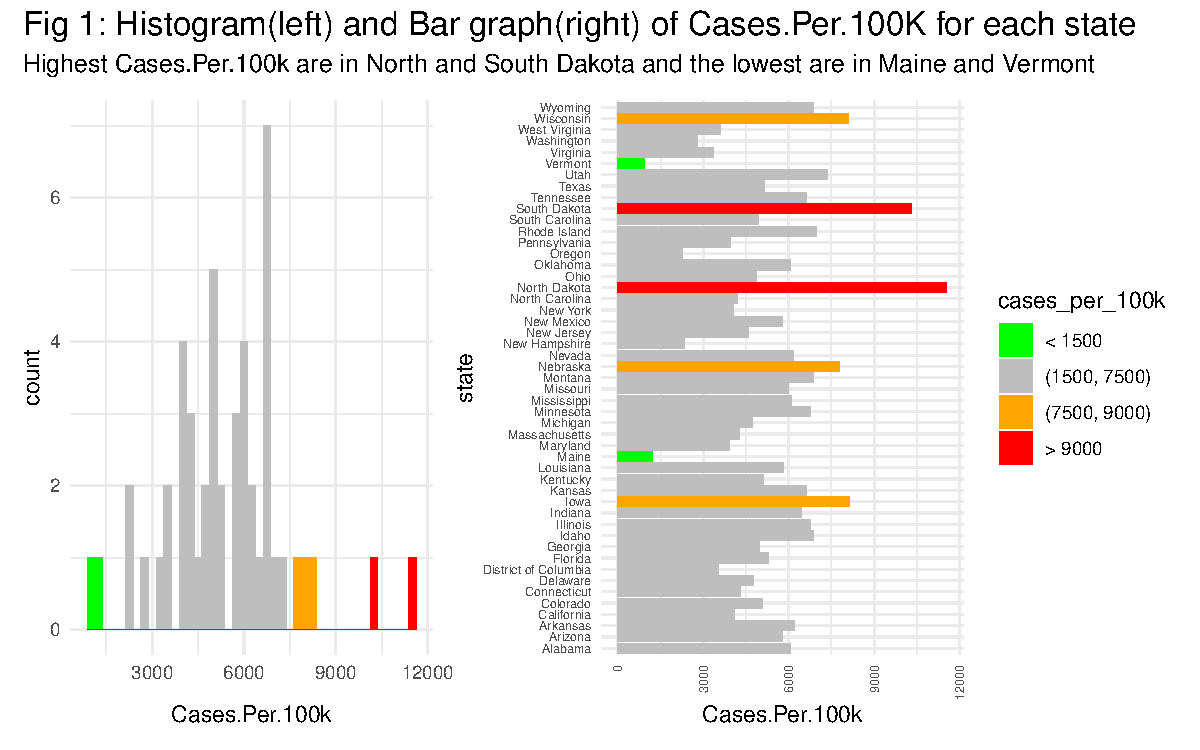
\includegraphics{Final_Report_files/figure-latex/cases_per_100k-1.pdf}

\hypertarget{primary-response-variable}{%
\subsubsection{Primary Response
Variable}\label{primary-response-variable}}

As we had described in the introduction section, we considered
`\textbf{\emph{Coronavirus-19 cases per hundred thousand residents}}' as
our primary response variables. We consider two states to be equally
affected by COVID, only if they have the same rate of occurrence of
COVID, i.e the number of COVID cases as a fraction of the total
populations is the same. We standardized the total cases per state into
total cases per 100,000 residents of state using the following formula:
\[
\text{Cases.Per.100K} = \frac{\text{cases}}{\text{Total.Population}}\times100,000
\]

The total number of cases per state is available as the variable `cases'
from the \emph{NYT COVID dataframe}. Each states population is available
as the variable `Total.Population' from the \emph{US Census dataframe}.
Both of these variables are described in detail in the data engineering
section. As the ratio \(cases/Total.Population\) represents the fraction
of population of COVID-19 cases, we multiply it by 100,000 to scale the
fraction to one hundred thousand residents. With this transformation
\emph{Cases.Per.100K} now represents the operationalized variable for
the primary response variables `Covid cases per one hundred thousand
residents'

\textbf{A discussion on the primary response variable}\\
\textbf{Fig 1(left)} shows the histogram of \emph{Cases.Per.100k}. We do
not observe heavy tails in the histogram of \emph{Cases.Per.100k}. We
identify two data points that are higher than the bulk of the
distribution and highlight them in red. Using the bar graph on
\textbf{Fig 1(right)} we identify those two points as the states, North
Dakota and South Dakota. Similarly, we identify two data points that are
lower than the bulk of the distribution and identify it as the state of
Maine and Vermont. We also take note of the states marked in orange that
are on the high of the bulk of the distribution of
\emph{Cases.Per.100k}. These states are Nebraska, Iowa and Wisconsin. As
these seven states are likely to have high leverage in the regression
models, we pay special attention to these while deciding on the
covariates.

\hypertarget{primary-explanatory-variables}{%
\subsubsection{Primary Explanatory
Variables:}\label{primary-explanatory-variables}}

\textbf{People of color:} As we had described in the introduction
section, we considered `percentage of People of color in the state
population' as one of our primary explanatory variables. We consider two
states to have equal representation of people of color only if the rate
of occurrence of people of color is the same, i.e.~the number of people
of color as a fraction of the total state population is the same. The
total population of a state, in percentages, can be summed as two
components, namely, percentage of people who identify as white only and
percentage of people who do not identify as white only . As we have
defined, in the introduction, that ``People of Color in the scope of
this research are defined as people who do not identify as belonging to
a white race only''; we calculate the percentage of the population of
people of color in the state population by subtracting the percentage of
the population who identify as white from one hundred percent.
Specifically,

\[
\text{Percent.People.Of.Color} = 100 -\text{Percent.White}
\]

With this transformation \emph{Percent.People.Of.Color} now represents
the operationalized variable for `percentage of the population of people
of color in the state population'

\textbf{Hispanic or latino:} As we had described in the introduction
section, we considered `percentage of Hispanic or Latino people in the
state population' as one of our primary explanatory variables. We
consider two states to have equal representation of Hispanic or Latino
people if the rate of occurrence of Hispanic or Latino people is the
same, i.e.~the number of Hispanic or Latino people as a fraction of the
total state population is the same. Hispanic or Latino as a demographic
is an ethnicity and not a race, i.e.~a person of Latin origin could
identify as white or any other race. Hence we included it as a separate
explanatory variable from persons of color. We used the variable
\emph{Percent.Hispanic.Or.Latino} from the \emph{US Census data frame}
without transformations for the operationalization of `percentage of
Hispanic or Latino people in the state population'.

\hypertarget{covariate-explanatory-variables}{%
\subsubsection{Covariate explanatory
variables}\label{covariate-explanatory-variables}}

As stated in the objective, the covariate variables are included to
provide context to the analysis. The key categories we had identified
and the corresponding variables are listed below. Note that the detailed
extraction of these from their corresponding datasets is in the data
engineering section.

\hypertarget{state-covid-policies-and-socioeconomic-conditions}{%
\paragraph{\texorpdfstring{State COVID Policies and Socioeconomic
Conditions:\\
}{State COVID Policies and Socioeconomic Conditions: }}\label{state-covid-policies-and-socioeconomic-conditions}}

The following variables were extracted from the State Policy dataframe
without any transformation:

\begin{enumerate}
\def\labelenumi{\arabic{enumi}.}
\tightlist
\item
  \emph{Days.Stay.At.Home}: Number of days stay at home order was issued
  in the time period of interest.
\item
  \emph{Days.With.Mask}: Number of days the mandate to wear a mask was
  on in the time period of interest.\\
\item
  \emph{Days.Restaurant.Closed}: Number of days restaurants were
  mandated to close in the time period of interest.
\item
  \emph{Days.Bar.Closed}: Number of days bars were mandated to close in
  the time period of interest.
\item
  \emph{Days.Gym.Closed}: Number of days Gyms were mandated to close in
  the time period of interest.
\item
  \emph{Days.Nonesst.bussi.Closed}: Number of days non-essential
  businesses were mandated to close in the time period of interest.
\item
  \emph{Percent.Poverty}: Percentage of population of the state below
  the poverty line.
\end{enumerate}

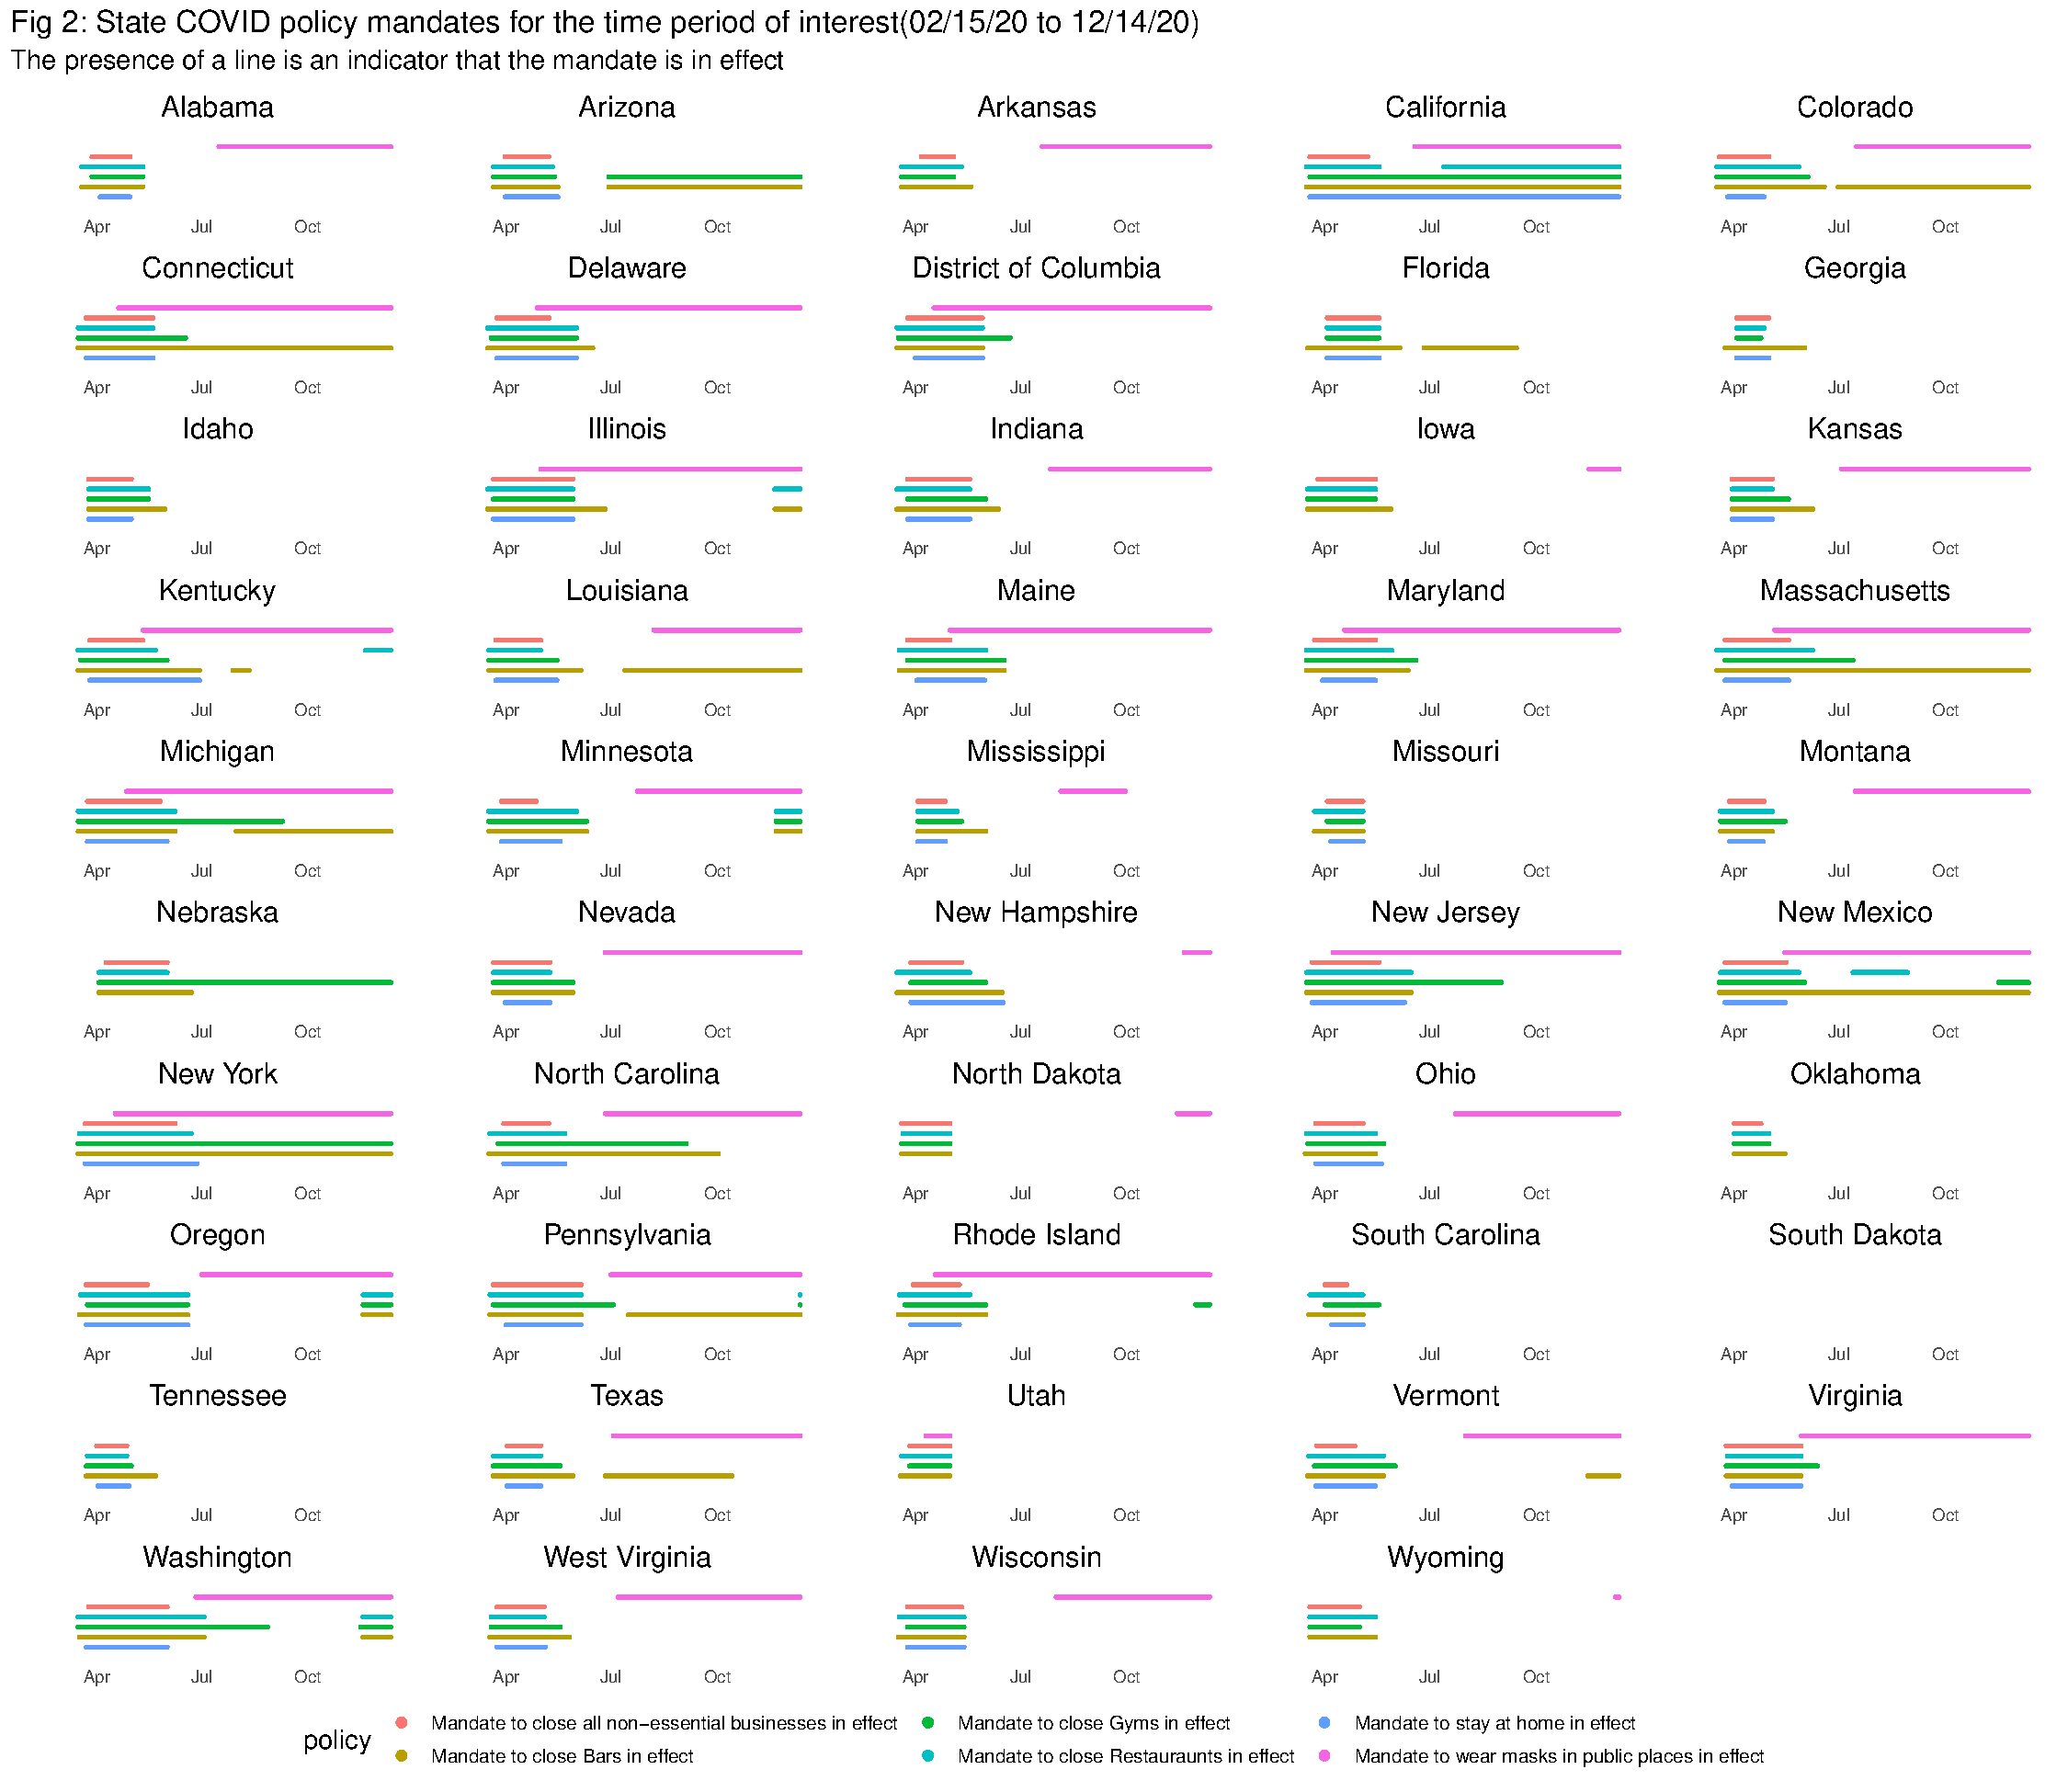
\includegraphics{Final_Report_files/figure-latex/unnamed-chunk-1-1.pdf}

\textbf{Fig 2} shows the timeline of when each State executed the
different mandates such as `stay at home' or `wearing masks in public
places'. In the discussion of the primary response variable (\textbf{Fig
1}) we had observed that North and South Dakota had high
\emph{Cases.Per.100k}. In \textbf{Fig 2} we observe that South Dakota
had not implemented any COVID related state mandates during the time
period of interest. North Dakota although did implement state mandates,
it was only for a short period of time relative to other states. Take
note that North Dakota did not implement Stay at Home order at any time
and the Mandate to wear masks was for a short time in the period of
interest. We had also noted in \textbf{Fig 1} states that were high in
\emph{Cases.Per.100k} but not as high as North and South Dakota. We had
marked them in orange and the states are Nebraska, Iowa and Wisconsin.
We note that neither Nebraska or Iowa implement a stay at home mandate.
The mask mandate was initiated for Iowa but only for a short time in the
period of interest. Wisconsin, on other hand, implemented a stay at home
mandate for a short period.We also observes that states such as
Washington and New Mexico had multiple phases of mandate implementation.
With these observations we make a qualitative assessment that the sum of
days a mandate was in effect in a state would provide useful information
for the model. We then expect that the operationalized variables for
stay at home order, i.e.~\emph{Days.Stay.At.Home} and for mask mandates,
i.e.~\emph{Days.With.Mask} would have an impact on
\emph{Covid.Cases.Per.100k}.

\hypertarget{google-community-mobility}{%
\paragraph{Google Community Mobility:}\label{google-community-mobility}}

The following variables were extracted from the Google Community
Mobility Estimates data frame without any transformation:

\begin{enumerate}
\def\labelenumi{\arabic{enumi}.}
\tightlist
\item
  \emph{Residential}: Average relative change in the length of stay at
  home during the time period of interest.
\item
  \emph{Workplace}: Average relative change in the length of stay at the
  workplace during the time period of interest.
\item
  \emph{Grocery}: Average relative change in the length of stay at the
  grocery or pharmacy during the time period of interest.
\item
  \emph{Parks}: Average relative change in the length of stay at the
  Park or areas of recreation during the time period of interest.
\item
  \emph{Transit}: Average relative change in the length of stay in
  transit stations, such as bus and train stops, during the time period
  of interest.
\end{enumerate}

\hypertarget{summary-table-of-all-variables}{%
\subsubsection{Summary table of all
variables}\label{summary-table-of-all-variables}}

\begin{table}[!h]

\caption{\label{tab:unnamed-chunk-2}Response, explanatory and covariate variables summary statistics and categories}
\centering
\begin{tabular}[t]{l|l|>{\raggedright\arraybackslash}p{3cm}|l|l|l}
\hline
variable & source & category & min & mean & max\\
\hline
Percent.Hispanic.Or.Latino & US Census Bureau & Socioeconomic (Primary explanatory) & 2 & 49 & 49\\
\hline
Recreation & Google communit mobility & Community mobility & -47 & -3 & -3\\
\hline
Grocery & Google communit mobility & Community mobility & -20 & 16 & 16\\
\hline
Parks & Google communit mobility & Community mobility & -34 & 153 & 153\\
\hline
Transit & Google communit mobility & Community mobility & -61 & 16 & 16\\
\hline
Workplace & Google communit mobility & Community mobility & -47 & -19 & -19\\
\hline
Residential & Google communit mobility & Community mobility & 5 & 16 & 16\\
\hline
Days.Stay.At.Home & US State Policy & State Policy & 0 & 270 & 270\\
\hline
Days.Restaurant.Closed & US State Policy & State Policy & 0 & 217 & 217\\
\hline
Days.Bar.Closed & US State Policy & State Policy & 0 & 273 & 273\\
\hline
Days.Gym.Closed & US State Policy & State Policy & 0 & 273 & 273\\
\hline
Days.Nonessential.Closed & US State Policy & State Policy & 0 & 78 & 78\\
\hline
Percent.Poverty & US State Policy & Socioeconomic & 8 & 20 & 20\\
\hline
Religious.Event.Exempt & US State Policy & State Policy & 0 & 1 & 1\\
\hline
Cases.Per.100k & NYT COVID/US Census & Primary response & 939 & 11557 & 11557\\
\hline
Percent.Person.Of.Color & US Census Bureau(transformed) & Socioeconomic (Primary explanatory) & 6 & 58 & 58\\
\hline
\end{tabular}
\end{table}

\hypertarget{variable-selection-for-model-development}{%
\subsection{Variable selection for model
development}\label{variable-selection-for-model-development}}

\textbf{Note on terminology: We use the category column in Table 8 to
describes variables in this section of the document}

\hypertarget{variables-for-model-1}{%
\subsubsection{Variables for model 1}\label{variables-for-model-1}}

As our objective for model 1 was to only includes our primary
explanatory variables \emph{Percent.People.Of.Color} and
\emph{Percent.Hispanic.Or.Latino}. We generated a scatter plot matrices
using the `psych' package in `R' to visualize the relationship between
\emph{Cases.Per.100k, Percent.People.Of.Color and
Percent.Hispanic.Or.Latino}.

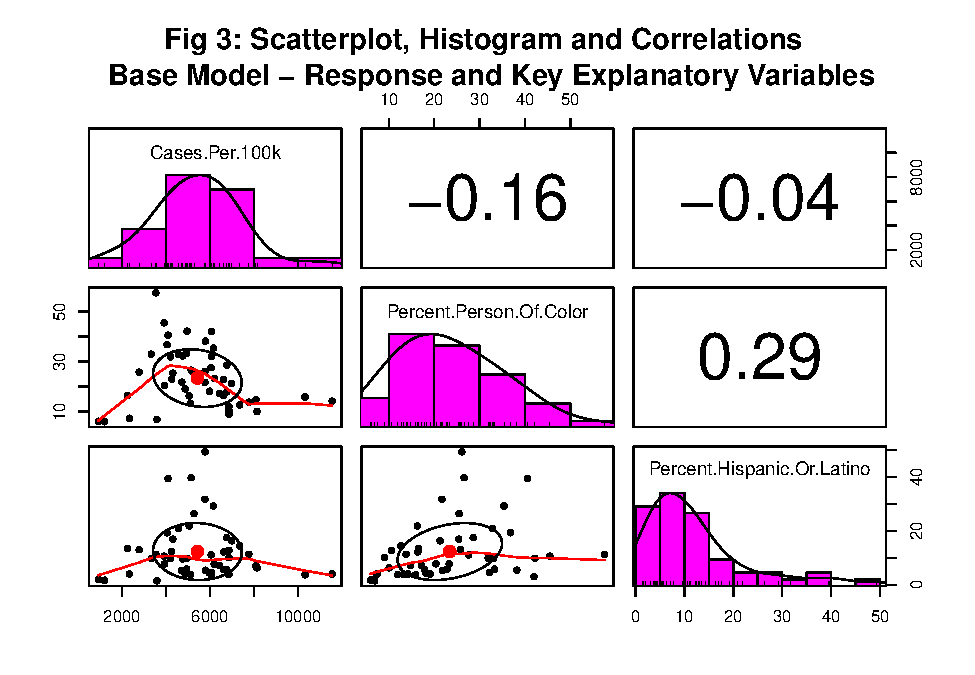
\includegraphics{Final_Report_files/figure-latex/unnamed-chunk-3-1.pdf}

As both of the explanatory variables did not demonstrate a nonlinear
relationship with \emph{Cases.Per.100k} in the scatterplot as seen in
\textbf{Fig 3}, and were well distributed without heavy tails in the
histogram in \textbf{Fig 3}, no transformations was required. The
Pearson's correlations coefficient between
\emph{Percent.Hispanic.Or.Latino} and \emph{Cases.Per.100K} and between
\emph{Percent.People.Of.Color} and \emph{Cases.Per.100K} were low on
their own.

\hypertarget{selection-of-covariates-for-model-2}{%
\subsubsection{Selection of Covariates for Model
2}\label{selection-of-covariates-for-model-2}}

We first combined the variable categories of State Policy and
Socioeconomic Conditions and analyzed them together. We treated the
community mobility variables on their own. We now generated two
additional scatter plot matrices using the `psych' package in `R', to
visualize the relationship between \emph{Cases.Per.100k} and the
covariate variables. We then used these scatter plots to identify
variables that have the strongest explanatory benefit to
\emph{Cases.Per.100k}. We also used the scatter plots to identify
transformations that may be required to address any non-linearities in
the relationships to \emph{Cases.Per.100k}. The two scatter plots are
\textbf{Fig 4} and \textbf{Fig 5}.

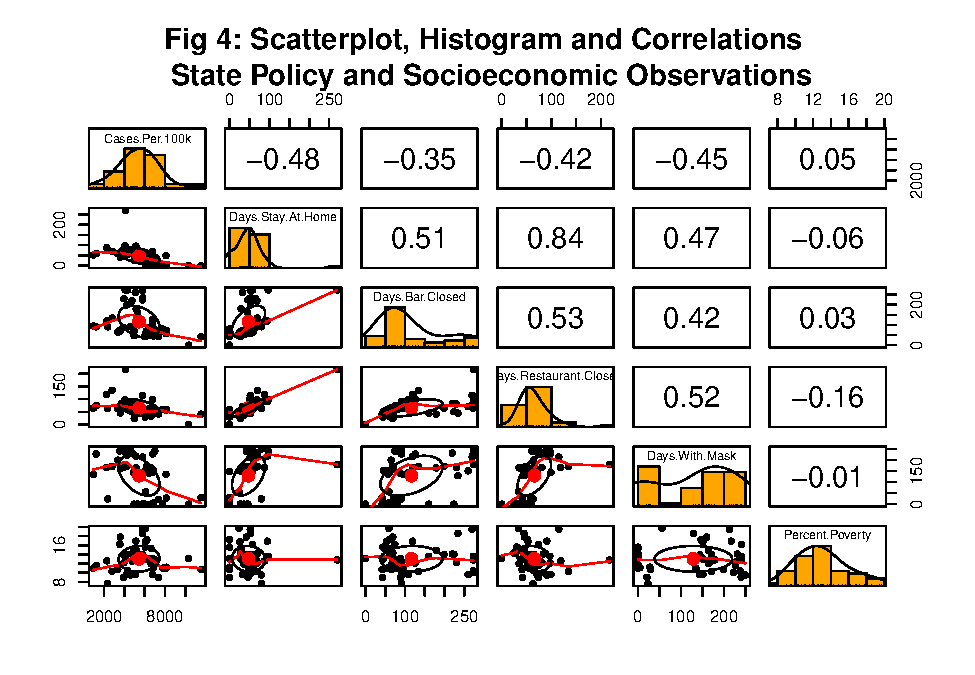
\includegraphics{Final_Report_files/figure-latex/psych-1-1.pdf}

As discussed in \textbf{section 3.13.1} we had hypothesized that among
the variables, we expected \emph{Days.Stay.At.Home} and
\emph{Days.With.Mask} to be the strongest predictors for
\emph{Cases.Per.100k}. Intuition tells us that when people were
isolating by staying at home there was reduced opportunity for virus
transmission and this variable hence encompasses all other restrictions.
Matching our expectation, upon viewing the scatterplot of correlations
in \textbf{Fig 4}, we found the highest correlation between
\emph{Cases.Per.100k} and the closure variables in this dataset was for
\emph{Days.Stay.At.Home} vs \emph{Cases.Per.100k}, hence we selected
this variable as a parameter for our main model. While the absolute
correlation factor of 0.46 was strongest, we noticed that there was
clustering in the data points. Since there were clustered values between
0 and 270 as seen in the histograms in \textbf{Fig 4}, we proceeded with
a square root transformation as a logarithmic transformation would not
be feasible. As checked whether the transformations improved the linear
relationship between \emph{Days.Stay.At.Home} and \emph{Cases.Per.100k}
by comparing the the Pearson correlation coefficient before and after
the transformation. We noted that the transformation increased the
correlation from 0.46 to 0.63. We also observed that although we
expected a relationship between poverty rate and infection rate, there
was no correlation found for this variable and the response variable
therefore, we did not include it in our models. Finally, for the
parsimony and explain-ability of the model we consider only the
\emph{Days.Stay.At.Home} covariate for model 2 and included the
remaining variables for model 3.

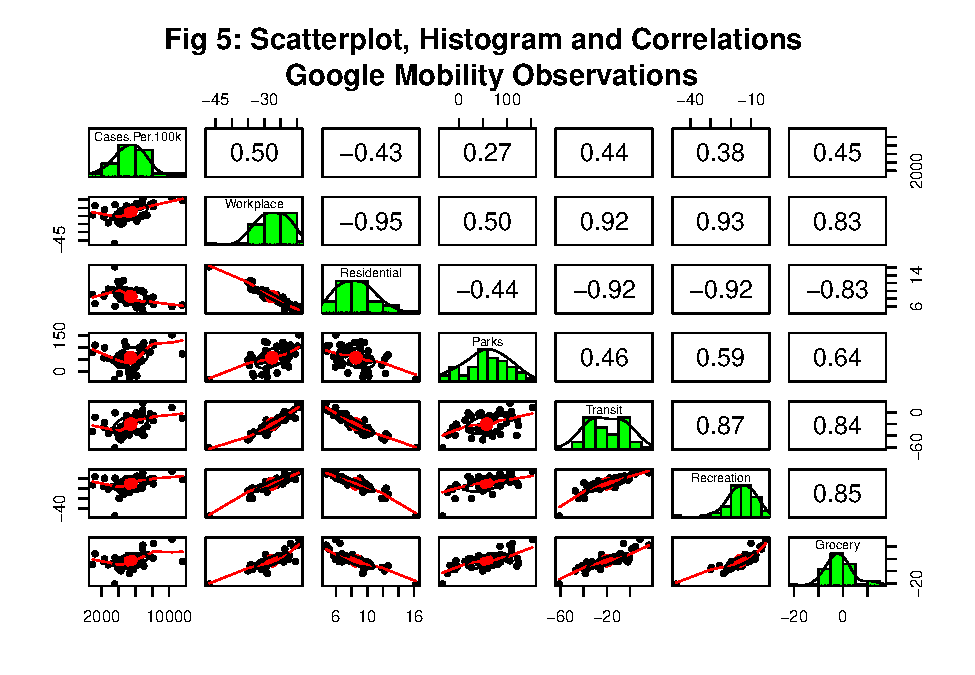
\includegraphics{Final_Report_files/figure-latex/psych-2-1.pdf}

Next we considered the Community Mobility category of variables from the
\emph{Google community mobility data frame}. When considering the
potential variables in the dataset, we expected \emph{Residential} and
\emph{Workplace} to be the two strongest indicators. The intuition we
followed was that most adults spend most time either at home or at work.
A greater than zero value for \emph{Residential} represents an increase
in time people spent at home. We expect an increase in
\emph{Residential} to be associated with a decrease in
\emph{Cases.Per.100k.} We also expect a correlation that an increase in
residential is inversely correlated with all other mobility parameters
such as workplace, parks etc.As more time spent at home is less time
spent in other locations.

Due to the physical interactions that are difficult to avoid in a
workplace environment, we expect an increase in \emph{Cases.Per.100k}
where \emph{Workplace} mobility was higher. While comparing these
explanatory variables with \emph{Cases.Per.100k}, we noticed that many
were moderately correlated with a Pearson's correlation coefficient
between 0.4 and 0.59 as seen in the correlation table \textbf{Fig 5},
and consistent with our expectation that a reduction in overall mobility
would also correlate to a reduction in infection rate. The most strongly
correlated variable we found in this dataset was \emph{Workplace}. As
this feature was strongly correlated, 0.80-0.95 with most other
variables in the dataset and highest correlated \emph{Cases.Per.100k} as
seen in figure 5, we selected this to be our next key variable from this
dataset. We did not choose \emph{Residential} for two reasons; first, we
had already included the \emph{Days.Stay.At.Home} from the State Policy
Dataset which is a similar indicator to residential mobility. As
stay-at-home mandate is asking people to stay more at home and
\emph{Residential} is the measured estimate of the same
parameter.Second, our objective was to create a parsimonious model with
good explainability and the high \emph{Residential} to \emph{Workplace}
correlation would not have allowed for that. As \emph{Workplace}
variable was evenly distributed and did not show a non-linearity with
\emph{Cases.Per.100k}, no transformation was performed on this variable.

\hypertarget{selection-of-covariates-for-model-3}{%
\subsubsection{Selection of Covariates for Model
3}\label{selection-of-covariates-for-model-3}}

As previously stated, the objective for model 3 is to produce the best
fit without the limitation of explaina-bility. To produce an improved
model we will add all of the community mobility variables and state
policy variables to the model. We validate the additions of these
variables in the model evaluation section.

\hypertarget{model-development}{%
\subsection{Model development}\label{model-development}}

For all of our model hypothesis testing we followed standard practice by
utilizing a maximum acceptance level with p-value of 0.05. A regression
table with all discussed results is provided following the model
section.

\hypertarget{model-1}{%
\subsubsection{Model 1}\label{model-1}}

Primary Response Variable:\\
* Cases per 100K Residents, (\emph{Cases.Per.100k})\\
Primary Explanatory Variables:\\
* Percentage Person of Color Residents,
(\emph{Percent.Person.Of.Color})\\
* Percentage Hispanic or Latino Residents,
(\emph{Percent.Hispanic.Or.Latino})\\

\textbf{Base model}
\[ \text{Cases per 100,000 Residents} = \beta_0 + \beta_1\times\text{Percent Person of Color} + \beta_2 \times \text{Percent Hispanic or Latino} + \epsilon \]
Following the standard practice of using a p-value of 0.05 we observe
the following hypotheses for our base model, as seen in the subsequent
regression table. Null Hypotheses:
\[H_0 : \beta_i = 0 \text{ Where i is the index for each coefficient of the regression equation}\]
Alternative Hypotheses:
\[H_A : \beta_i \neq 0, \text{ Where i is the index for each coefficient of the regression equation}\]

As required for model 1 of this study, our base model only includes our
primary explanatory variables, but does not show any statistical
significance based on our standard practice of an acceptance criteria
p-value of 0.05 and has an adjusted R-squared value of -0.17 as seen in
Regression Table as \textbf{Fig 6}. As none of our covariate's
coefficients showed a p-value \(\leq\) 0.05, we fail to reject the null
hypothesis that the coefficients are not 0. Although not statistically
significant, this model was a crucial starting point for bringing in the
key variables that are needed to reject or fail to reject the null
hypothesis that a State's increased percentage of People of Color and
Hispanic or Latino residents has no difference in the rate of
coronavirus spread.

\hypertarget{model-2}{%
\subsubsection{Model 2}\label{model-2}}

Primary Response Variables:\\
* Cases per 100K Residents (\emph{Cases.Per.100k})\\
Primary Explanatory Variables:\\
* Percentage Person of Color Residents
(\emph{Percent.People.Of.Color})\\
* Percentage Hispanic or Latino Residents
(\emph{Percent.Hispanic.Or.Latino})\\
Additional Covariates:\\
* Workplace Mobility change from Baseline (\emph{Workplace})\\
* Square Root of Days with Stay at Home Order in effect
\(\sqrt{Days.Stay.At.Home}\)\\

\textbf{Improved model}
\[\text{Cases per 100,000 Residents} = \beta_0 + \beta_1 \times \text{Percent Person of Color} +\]
\[\beta_2 \times \text{Percent Hispanic or Latino} +  \beta_3 \times \text{Workplace Mobility} + \beta_4 \times \sqrt{\text{Days Stay at Home}} + \epsilon \]

\begin{verbatim}
## Model 2 VIF Test Maximum:
\end{verbatim}

\begin{verbatim}
## [1] 2.192514
\end{verbatim}

First we conducted a Value Inflation Factor (VIF) test, which measures
how much the variance of a regression coefficient is inflated due to
multicollinearity in the model, using the guideline threshold value of 4
indicating strong collinearity between our covariates. The resulting
maximum value found was 2.193 which does not indicate perfect or nearly
perfect collinearity and allows us to continue the evaluation.

Following the standard practice of using a p-value of 0.05 we observe
the following hypotheses for our second model, as seen in the following
regression table. Null Hypotheses:
\[H_0 : \beta_i = 0 \text{ Where i is the index for each coefficient of the regression equation}\]
Alternative Hypotheses:
\[H_A : \beta_i \neq 0, \text{ Where i is the index for each coefficient of the regression equation}\]
This model brought considerable improvement in our covariate's
significance. Using our previously stated acceptance criteria of a
p-value \(\le\) 0.05, we detected statistical significance on
\(\beta_2 = 46.069\), \(\beta_3 = 164.157\) and \(\beta_ 4 = -315.922\),
giving a final model of:

\[ \text{Cases per 100,000 Residents} = 10,656.500 + 29.121 \times \text{Percent.Person.Of.Color} + \]
\[46.069 \times \text{Percent Hispanic or Latino} +  164.157 \times \text{Workplace Mobility} -315.922 \times \sqrt{ \text{Days Stay at Home}} + \epsilon\]

Model 2 was a much better fit for the population as our adjusted
R-squared value increased from -0.17 to 0.451 as seen in the Regression
Table in \textbf{Fig 6}. Although we did not see significance in the
features representing the percentage of persons of color
(\emph{Percent.Person.Of.Color}) variable, the standard errors on all
variables were greatly reduced.

Finally, we conducted an Analysis of Variance between Model 1 and Model
2 with our standard p-value criteria of 0.05. For the ANOVA test, we use
a null hypothesis that there is no improvement in performance from the
inclusion of the added variables in Model 2 vs Model 1 alternative
hypothesis that there is an improvement between iterations.

\begin{verbatim}
## Analysis of Variance Table
## 
## Model 1: Cases.Per.100k ~ 1 + Percent.Person.Of.Color + Percent.Hispanic.Or.Latino
## Model 2: Cases.Per.100k ~ 1 + Percent.Person.Of.Color + Percent.Hispanic.Or.Latino + 
##     Workplace + sqrt(Days.Stay.At.Home)
##   Res.Df       RSS Df Sum of Sq      F    Pr(>F)    
## 1     46 190081681                                  
## 2     44  98229931  2  91851750 20.572 4.928e-07 ***
## ---
## Signif. codes:  0 '***' 0.001 '**' 0.01 '*' 0.05 '.' 0.1 ' ' 1
\end{verbatim}

Conducting this test(test results above), we observed an F score of
20.572 that corresponds to a p-value of 4.928e-07 which rejects the null
hypothesis that there is no improvement between Model 1 and Model 2.

With the confirmation that there is an improvement between the models'
performance we can now address what this model conveys. To interpret the
meaning of this model, each variable must be looked at independently. As
the minimum value of the percent Hispanic or Latino variable is 1.5\%
and this includes the entire population in question, the intercept term
may never be met on its own with all explanatory variables at 0 and
therefore does not have a valid independent interpretation within the
bounds of this model. It can only be used to explain the overall model
relationships. When reviewing the remaining explanatory variables, all
covariate impact to the \emph{Cases.Per.100k} may be reviewed
independently under the guideline that all other variables are to remain
unchanged(\emph{Ceteris Paribus}).

\begin{enumerate}
\def\labelenumi{\arabic{enumi}.}
\tightlist
\item
  The coefficient \(\beta_1 = 29.121\) represents an increased infection
  rate of 29.121 \emph{Cases.Per.100k} residents if
  \emph{Percent.People.Of.Color} in a state is increased by 1 unit while
  all other variables are unchanged. As the unit of
  \emph{Percent.People.Of.Color} is percentage, a 1 unit increase
  represents a 1\% increase in people of color as a fraction of the
  state population.
\item
  Coefficient \(\beta_2 = 46.069\) represents an increased infection
  rate of 46.069 \emph{Cases.Per.100k} residents if
  \emph{Percent.Hispanic.Or.Latino} is increased in a state by 1 keeping
  all else equal. As the unit of \emph{Percent.Hispanic.Or.Latino} is
  percentage, a 1 unit increase represents a 1\% increase in Hispanic or
  Latino as a fraction of the state population.
\item
  Coefficient \(\beta_3 = 164.157\) represents an increase of 164.157
  \emph{Cases.Per.100k} residents if the residents spend an extra 1
  percent of their time at work relative to the baseline, keeping all
  other variables unchanged. This aligns with our expectation that more
  people physically attending workplaces is associated with an increase
  in Covid cases.
\item
  Finally, \(\beta_4 = -315.922\). This represents a decrease in
  \emph{Cases.Per.100k} with increase in \emph{Days.Stay.At.Home} which
  is the total days that a stay at home order was in place for each
  state. As the covariate has a square root relationship with the
  response, we make the following numeric approximation to describe the
  relationship; a 10\% increase in \emph{Days.Stay.At.Home} is
  associated with a \(0.7 \times 315.922 \times 0.1 = 22.1\) decrease in
  \emph{Cases.Per.100k} residents.This aligns closely with the intuition
  that isolation would reduce the spread of COVID-19.
\end{enumerate}

\hypertarget{model-3}{%
\subsubsection{Model 3}\label{model-3}}

Although model 2 provided a good fit and described the relationship
between the variables belonging to the overall population, we then
search for an improved model that provided an even better fit without
the need for explain-ability. In addition to the parameters of model 2
we included:

\begin{enumerate}
\def\labelenumi{\arabic{enumi}.}
\tightlist
\item
  Square root of days that a mask mandate: \emph{Days.With.Mask} was in
  place
\item
  All of the remaining closure parameters that were not included in
  model 2 as a single term that is the summation of the square roots of
  each closure term: \emph{Days.Bar.Closed},
  \emph{Days.Restaurant.Closed}, \emph{Days.Gym.Closed}, and
  \emph{Days.Nonessential}
\item
  A square root transformation was used for all variables within the
  State Policy dataset as we saw strong clustering and wide
  distributions between states.
\item
  By performing this transformation and including the total of all
  mandate durations, we were able to create a random variable which was
  heavily weighted to states with a more aggressive response to COVID,
  i.e.~more total closure days for every category of closure. that
  proved effective in isolating state behaviors.
\item
  Finally, we included the remaining mobility terms. As the remaining
  mobility values: \emph{Parks}, \emph{Recreation}, \emph{Residential},
  \emph{Transit} and \emph{Grocery}, were a combination of negative and
  positive values, we took the square of each and summed them together
  into a single mobility term.
\end{enumerate}

These additional variables gave us a final model of:
\[ \text{Cases.Per.100k} = 9,545.145 + 63.112\times\text{Percent.People.Of.Color} + \ 63.342\times\text{Percent.Hispanic.Or.Latino} + \]
\[ 206.339 \times \text{Workplace} -292.031\times\sqrt{\text{Days.Stay.At.Home}} -7.933\times\sqrt{\text{Days.With.Mask}} + \]
\[0.150\times\Bigg({\text{Residential}^2 + \text{Grocery}^2 +  \text{Recreation}^2 + \text{Parks}^2 + \text{Transit}^2}\Bigg) +\]
\[ 7.469\times\Bigg({\sqrt{\text{Days.Gym.Closed}} + \sqrt{\text{Days.Bar.Closed}} + \sqrt{\text{Days.Restaurant.Closed}} + \sqrt{\text{Days.Nonessential.Closed}}}\Bigg) +\epsilon\]

After incorporating these remaining features we verified that there was
no strong collinearity by conducting a value inflation factor test with
the guideline that a VIF of 4 or larger represents strong collinearity.
The test provided a resulting maximum value of 2.848 validating the
assumption that the variables were neither perfectly nor nearly
collinear.

\begin{verbatim}
## Model 3 VIF Test Maximum:
\end{verbatim}

\begin{verbatim}
## [1] 2.84885
\end{verbatim}

To build confidence in our model, we validated if the added variables
impacted our model by once again conducting an ANOVA F-test between
Model 2 and Model 3. We followed standard practice and set a threshold
p-value of 0.05, with a null hypothesis that there was no improvement
with the addition of more variables from model 2 and model 3 and an
alternative hypothesis that there was an improvement found with the
inclusion of the added variables between Models 2 and 3.

\begin{verbatim}
## Analysis of Variance Table
## 
## Model 1: Cases.Per.100k ~ 1 + Percent.Person.Of.Color + Percent.Hispanic.Or.Latino + 
##     Workplace + sqrt(Days.Stay.At.Home)
## Model 2: Cases.Per.100k ~ 1 + Percent.Person.Of.Color + Percent.Hispanic.Or.Latino + 
##     Workplace + sqrt(Days.Stay.At.Home) + sqrt(Days.With.Mask) + 
##     I(Residential^2 + Grocery^2 + Recreation^2 + Parks^2 + Transit^2) + 
##     I(sqrt(Days.Gym.Closed) + sqrt(Days.Bar.Closed) + sqrt(Days.Restaurant.Closed) + 
##         sqrt(Days.Nonessential.Closed))
##   Res.Df      RSS Df Sum of Sq     F Pr(>F)  
## 1     44 98229931                            
## 2     41 80154370  3  18075561 3.082 0.0378 *
## ---
## Signif. codes:  0 '***' 0.001 '**' 0.01 '*' 0.05 '.' 0.1 ' ' 1
\end{verbatim}

The F-test generated(test results above) an F-statistic of 3.092 and a
p-value of 0.0378, again rejecting the null hypothesis that there was no
improvement in our model 3 iteration. As seen in the \textbf{Fig 6}
generated using the Stargazer package, the adjusted R-Squared value was
increased from 0.451 in model 2 to 0.519 for model 3 confirming that the
model prediction was improved with these additional parameters.

To evaluate the coefficients we again follow the standard practice of
using a p-value of 0.05 we observe the following hypotheses for our
third model: Null Hypotheses:
\[H_0 : \beta_i = 0 \text{ Where i is the index for each coefficient of the regression equation}\]
Alternative Hypotheses:
\[H_A : \beta_i \neq 0, \text{ Where i is the index for each coefficient of the regression equation}\]

In our hypothesis testing, as seen in the following regression
table\textbf{(Fig 6)}, we found statistical significance to reject the
null hypothesis for \(\beta_0\), \(\beta_1\), \(\beta_2\), \(\beta_3\),
\(\beta_4\), and \(\beta_5\). Therefore, we conclude that
\(\beta_0 = 9,545.145\), \(\beta_1 = 63.112\), \(\beta_2 = 63.342\),
\(\beta_3 = 206.339\), \(\beta_4 = -292.031\), \(\beta_6 = 0.150\) which
can all be found in our regression table in \textbf{Fig 6} below. This
left us with a final model of:
\[\text{Cases.Per.100k} = 9,545.145 + 63.112\times\text{Percent.People.Of.Color} + 63.342\times\text{Percent.Hispanic.Or.Latino} +\]
\[206.339 \times \text{Workplace}   -292.031\times\sqrt{\text{Days.Stay.At.Home}} -7.933\times\sqrt{Days.With.Mask} +\]
\[0.150\times\sum\Bigg({Residential^2, Grocery^2,  Recreation^2, Parks^2, Transit^2}\Bigg) +\]
\[7.469\times\sum\Bigg({\sqrt{Days.Gym.Closed} , \sqrt{Days.Bar.Closed} , \sqrt{Days.Restaurant.Closed} , \sqrt{Days.Nonessential.Closed}}\Bigg) +\epsilon\]

\hypertarget{model-regression-table}{%
\subsubsection{Model Regression Table}\label{model-regression-table}}

\textbf{Fig 6: SARS Coronavirus-19 Cases per 100,000 Residents Covariate
Regression Table using Classic Standard Errors}

\begingroup 
\footnotesize 
\begin{tabular}{@{\extracolsep{1pt}}lccc} 
\\[-1.8ex]\hline 
\hline \\[-1.8ex] 
 & \multicolumn{3}{c}{\textit{Dependent variable:}} \\ 
\cline{2-4} 
\\[-1.8ex] & \multicolumn{3}{c}{Reported Coronavirus-19 Cases per 100,000 Residents} \\ 
 & Base Model & Efficient Model & Best Fit Model \\ 
\\[-1.8ex] & (1) & (2) & (3)\\ 
\hline \\[-1.8ex] 
 Intercept & 6,075.423 & 10,656.500 & 9,545.145 \\ 
  & (686.648)$^{***}$ & (1,286.931)$^{***}$ & (1,358.792)$^{***}$ \\ 
  & p = 0.000 & p = 0.000 & p = 0.00000 \\ 
  State - Percentage of Residents People of Color & $-$28.295 & 29.121 & 63.112 \\ 
  & (26.580) & (22.991) & (25.760)$^{**}$ \\ 
  & p = 0.293 & p = 0.212 & p = 0.019 \\ 
  State - Percentage of Residents Hispanic or Latino & 1.904 & 46.069 & 64.342 \\ 
  & (28.985) & (22.787)$^{**}$ & (23.305)$^{***}$ \\ 
  & p = 0.948 & p = 0.050 & p = 0.009 \\ 
  Workplace Mobility Impact &  & 164.157 & 206.339 \\ 
  &  & (62.347)$^{**}$ & (66.493)$^{***}$ \\ 
  &  & p = 0.012 & p = 0.004 \\ 
  Square Root of Days State was Under Stay at Home Order &  & $-$315.922 & $-$292.031 \\ 
  &  & (79.847)$^{***}$ & (89.657)$^{***}$ \\ 
  &  & p = 0.0003 & p = 0.003 \\ 
  Square Root of Days with Mask Mandate &  &  & $-$7.933 \\ 
  &  &  & (45.154) \\ 
  &  &  & p = 0.862 \\ 
  Sum of Squares, All Other Mobility Scores &  &  & 0.150 \\ 
  &  &  & (0.051)$^{***}$ \\ 
  &  &  & p = 0.006 \\ 
  Sum of Square Roots, All Other Closures &  &  & 7.469 \\ 
  &  &  & (37.760) \\ 
  &  &  & p = 0.845 \\ 
 \hline \\[-1.8ex] 
Observations & 49 & 49 & 49 \\ 
R$^{2}$ & 0.025 & 0.496 & 0.589 \\ 
Adjusted R$^{2}$ & $-$0.017 & 0.451 & 0.519 \\ 
Residual Std. Error & 2,032.784 (df = 46) & 1,494.155 (df = 44) & 1,398.208 (df = 41) \\ 
\hline 
\hline \\[-1.8ex] 
\textit{Note:}  & \multicolumn{3}{r}{$^{*}$p$<$0.1; $^{**}$p$<$0.05; $^{***}$p$<$0.01} \\ 
\end{tabular} 
\endgroup

\hypertarget{discussion-on-causality}{%
\paragraph{Discussion on causality}\label{discussion-on-causality}}

The reader would note that the authors did not make causal claims in the
discussion of the models.

\begin{enumerate}
\def\labelenumi{\arabic{enumi}.}
\tightlist
\item
  Elaborating on the observation that ``an increase in the hispanic
  population is associated with an increase in cases per 100k''; there
  could be several underlying reasons for this association. One relating
  to the Socioeconomic status is the jobs held by people who identify as
  hispanic or Latino could also play a role in this association.
  Specifically, occupying jobs that require physical presence could
  increase the chances of the spread of COVID among this demographic. We
  have discussed this variable in the omitted variable section.
\item
  As physical isolation reduces the spread of
  COVID\textsuperscript{{[}12{]}}, we would then expect that the claim
  that the ``increase in \emph{Days.Stay.At.Home} is associated with a
  decrease in \emph{Cases.Per.100k}'' could be considered a causal
  relationship.
\item
  As physical proximity increases the spread of
  COVID\textsuperscript{{[}12{]}}, we would then expect that the claim
  that the ``increase in \emph{Workplace} is associated with an increase
  in \emph{Cases.Per.100k}'' could also be considered a causal
  relationship.
\end{enumerate}

\hypertarget{dicussion-on-the-assumption-for-the-classical-linear-model}{%
\subsection{Dicussion on the assumption for the Classical Linear
Model}\label{dicussion-on-the-assumption-for-the-classical-linear-model}}

\textbf{In this section we only discuss model 2 assumptions}\\

\hypertarget{iid}{%
\subsubsection{IID}\label{iid}}

\hypertarget{independence}{%
\paragraph{Independence}\label{independence}}

With respect to independence, let's recall that independence relates to
how we define our population and the process by which the samples are
obtained. In this case we are not using random selection since we are
using the entire population (all contiguous U.S. states and Washington
DC). As such, there might be clustering between states due to their
geographical location. In all cases, states are connected to at least
one other, and the virus can be spread across open borders, especially
to neighbors. States with more lenient restrictions such, as South
Dakota where no mask mandates were ever set in place, can spread the
virus to other states even if the other states enacted a statewide order
such as North Dakota\textsuperscript{{[}7{]}} From the map \textbf{Fig
7} we can see how both states have cases in the same range. Similarly,
Oregon and Washington state also have cases in the same range.\\

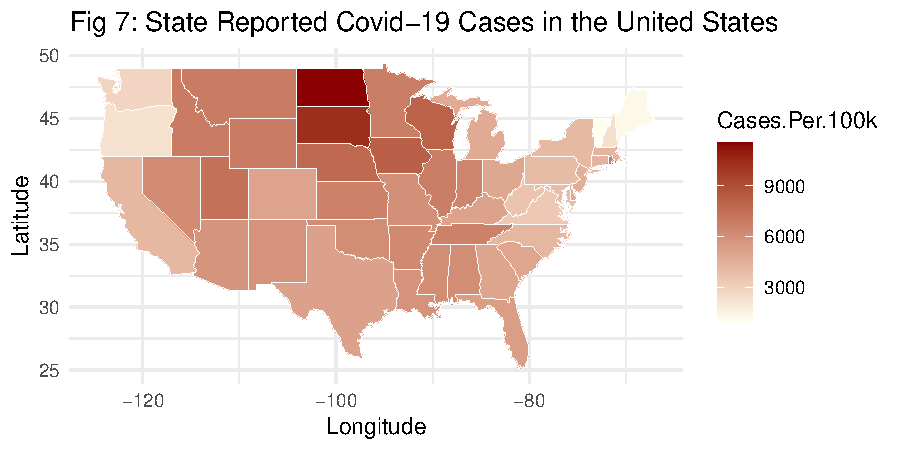
\includegraphics{Final_Report_files/figure-latex/iid-1.pdf} Dr.~Ashish
Jha, dean of the Brown University School of Public Health said: ``In
some ways, the whole country is essentially living with the strategy of
the least effective states because states interconnect and one state not
doing a good job will continue to spread the virus to other
states,''\textsuperscript{{[}8{]}}. Despite the CDC recommendations,
people are still travelling from low COVID-19 positivity rates states to
states with high positivity rates either for leisure or work related
which can expose them to COVID-19, and therefore spread the virus to
loved ones when they return back home.

\hypertarget{identically-distributed}{%
\paragraph{Identically Distributed}\label{identically-distributed}}

With respect to the Identically distributed assumption, it refers to all
observations coming from the same distribution, however each state is
responsible to collect their own data, but some are reporting inaccurate
results\textsuperscript{{[}9{]}}. In addition, not all states have the
same testing levels, which can cause sick people not getting tested and
consequently they might have a lower number of cases than states with
higher testing rates. Thus, the identical distribution assumption might
not hold either. Therefore, our observations fail to meet the IID
assumption. Because our observations didn't meet the IID assumption, our
OLS regression model might produce estimates that are biased.

\hypertarget{linear-conditional-mean}{%
\subsubsection{Linear conditional mean}\label{linear-conditional-mean}}

In order to test this assumption, we plot model the model prediction for
the fitted values and the corresponding residuals as a sctter plot
\textbf{Fig 8}

\textbf{Fig 8: Fitted values Vs Residuals}\\
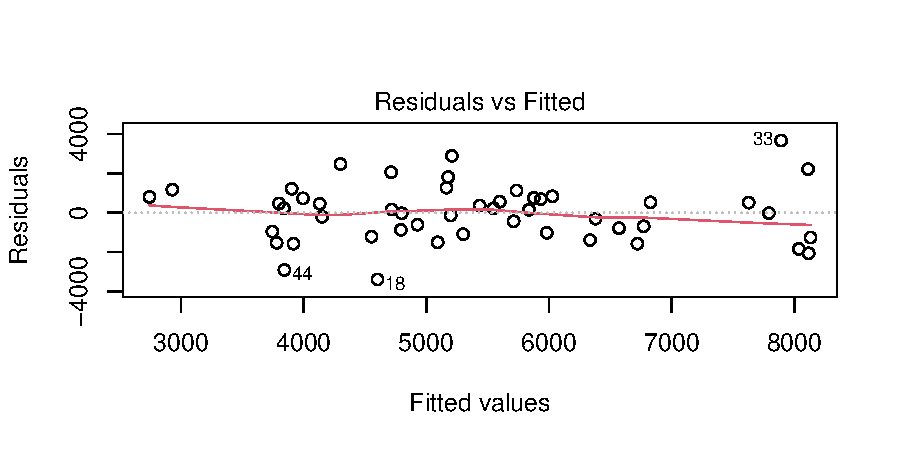
\includegraphics{Final_Report_files/figure-latex/lce-1.pdf}

As we can see from the plot above, the residuals bounce randomly around
the y=0 line. Since we don't see evidence of non-linearity, the
assumption that the relationship is linear is reasonable.

\hypertarget{no-perfect-collinearity}{%
\subsubsection{No perfect collinearity}\label{no-perfect-collinearity}}

In the presence of multicollinearity, the solution of the regression
model becomes unstable. Since our regression model didn't drop a
coefficient, we don't have perfect collinearity.

\begin{verbatim}
##                (Intercept)    Percent.Person.Of.Color 
##                10656.49932                   29.12132 
## Percent.Hispanic.Or.Latino                  Workplace 
##                   46.06886                  164.15653 
##    sqrt(Days.Stay.At.Home) 
##                 -315.92175
\end{verbatim}

We are also going to compute the variance inflation factor (VIF) which
measures how much the variance of a regression coefficient is inflated
due to multicollinearity in the model. We are using the guideline that a
VIF of 4 or larger represents strong collinearity.

\begin{verbatim}
##    Percent.Person.Of.Color Percent.Hispanic.Or.Latino 
##                   1.510818                   1.247972 
##                  Workplace    sqrt(Days.Stay.At.Home) 
##                   2.192514                   1.464738
\end{verbatim}

For \emph{Percent.People.Of.Color} we got a value of 1.51 which means
that the standard error for its respective coefficient is
\(\sqrt {1.51}\approx 1.22\) times larger than if
\emph{Percent.People.Of.Color} had 0 correlation with the other
predictor variables.

For \emph{Percent.Hispanic.Or.Latino} we got a value of 1.29 which means
that the standard error for its respective coefficient is
\(\sqrt {1.25} \approx 1.11\) times larger than if
\emph{Percent.Hispanic.Or.Latino} had 0 correlation with the other
predictor variables.

For \emph{Workplace} we got a value of 1.93 which means that the
standard error for its respective coefficient is
\(\sqrt {2.19} \approx 1.48\) times larger than if Workplace had 0
correlation with the other predictor variables.

For \(\sqrt{\text{Days.Stay.At.Home}}\) we got a value of 1.36 which
means that the standard error for its respective coefficient is
\(\sqrt {1.46} \approx 1.21\) times larger than if
\(\sqrt{Days.Stay.At.Home}\) had 0 correlation with the other predictor
variables.

Because all of these VIF scores are smaller than 4, they indicate
absence of multicollinearity. Thus, our model meets the ``No perfect
collinearity'' assumption.

\hypertarget{homoskedasticity}{%
\subsubsection{Homoskedasticity}\label{homoskedasticity}}

This assumption help us to determine the validity of our standard
errors. One way to test homeskedasticity is to examine the
scale-location plot \textbf{Fig 9}. Homoskedasticity would show up on
this plot as a flat smoothing curve.\\

\textbf{Fig 9: Scale location plot}\\
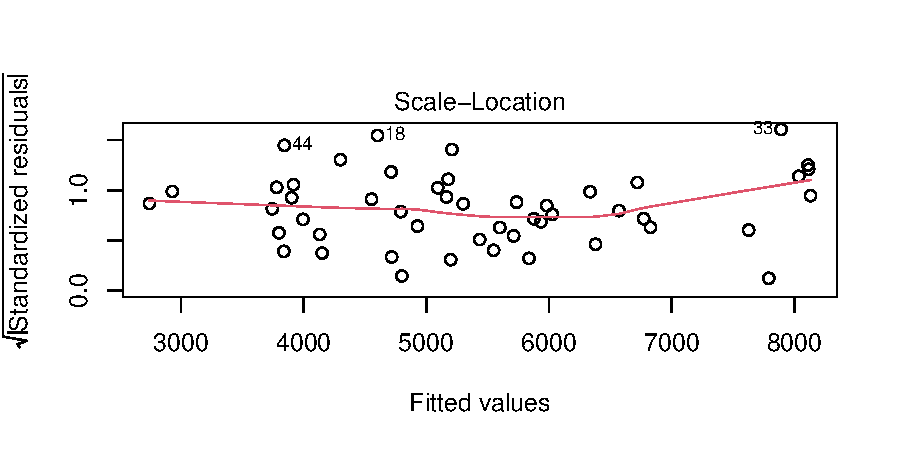
\includegraphics{Final_Report_files/figure-latex/hms-1.pdf}

There seems to be a deep increase for fitted values greater than 6000,
suggesting a problem with heteroskedasticity. In order to confirm this,
we are running a Breusch-Pagan test from the \texttt{lmtest} package the
\texttt{bptest} function. We follow standard practice and use a
significance level of 0.05.

\[H_o: \text{There is no evidence for heteroskedastic error variance (homoskedasticity)}\]
\[H_a: \text{There is heteroskedasticity}\]

\begin{verbatim}
## 
##  studentized Breusch-Pagan test
## 
## data:  model_2
## BP = 8.0811, df = 4, p-value = 0.08865
\end{verbatim}

Because our p-value = 0.09 \textgreater{} 0.05, we fail to reject our
null hypothesis that there is no evidence for heteroskedastic error
variance, so we conclude that we don't have evidence of heteroskedastic
error variance.

\hypertarget{normally-distributed-error}{%
\subsubsection{Normally distributed
error}\label{normally-distributed-error}}

We follow standard practice and use a significance level of 0.05. We are
also performing a Shapiro-Wilk's test, which is based on the correlation
between the data and the corresponding normal scores with
\[H_o: \text{residual errors are normally distributed}\]
\[H_a: \text{residual errors are not normally distributed}\]

\begin{verbatim}
## 
##  Shapiro-Wilk normality test
## 
## data:  model_2$residuals
## W = 0.98968, p-value = 0.9422
\end{verbatim}

Because our p-value = 0.94 \textgreater{} 0.05, we fail to reject our
null hypothesis which implies that there is no evidence that shows that
residual errors are not different from a normal distribution. Therefore,
the ``Normally Distributed Errors'' assumption holds, and we can trust
the t-value and p-value for every coefficient.

\hypertarget{discussion-on-confidence-intervals}{%
\subsection{Discussion on confidence
intervals}\label{discussion-on-confidence-intervals}}

\textbf{95\% Confidence Intervals:}

\begin{verbatim}
##                                  2.5 %      97.5 %
## (Intercept)                8062.859929 13250.13871
## Percent.Person.Of.Color     -17.214401    75.45704
## Percent.Hispanic.Or.Latino    0.145103    91.99262
## Workplace                    38.503960   289.80910
## sqrt(Days.Stay.At.Home)    -476.842784  -155.00072
\end{verbatim}

\(\beta_{\text{Percent.People.Of.Color}}\): We are 95\% confident that
the coefficient of Percent of People of Color is between -17.21 and
75.46. Since the confidence interval contains 0, we can conclude there
is no significant evidence of a linear relationship between
Percent.People.Of.Color and Cases.Per.100k, just like we found in the
model results.

\(\beta_{\text{Percent.Hispanic.Or.Latino}}\): We are 95\% confident
that the coefficient of State-Percentage of Residents Hispanic or Latino
is between 0.15 and 91.99.

\(\beta_{\text{Workplace}}\): We are 95\% confident that the coefficient
of Workplace Mobility is between 38.51 and 289.81.

\(\beta_{\sqrt{Days.Stay.At.Home}}\): We are 95\% confident that the
coefficient of Square Root of Days is between -476.84 and -155.00.

\hypertarget{limitations-of-the-model}{%
\section{Limitations of the model}\label{limitations-of-the-model}}

\hypertarget{limitations-in-data}{%
\subsection{Limitations in data}\label{limitations-in-data}}

We called out specific limitations that existed for the individual data
sets used to build the model in section 2.2. We will discuss these
limitations with respect to the primary response variables and the
primary explanatory variables selected to build the model.

The primary explanatory variable Cases.Per.100k as defined in section
3.1.1 is sourced from `cases' in the NY Times Covid Dataset and `Total
Population' in the US Census data frame.

1.For the NYT Times Dataset, we called out that certain states reported
confirmed cases while other states reported confirmed and probable
cases. This is a limitation of the data that adds to the error term to
the model. 2. The number of reported cases were also affected by the
testing rate and testing availability in each state.This is a limitation
of the data that adds to the error term to the model. 3. The rate of
spread of COVID within a state changed dramatically during a given
period, with spikes during periods associated with spring break or US
holidays. This could introduce variability to the analysis that could
not be explained with the analyzed variables. We mitigated this risk by
using a long time period for the analysis of 304 days.

We had noted that the US Census dataset was an estimate based on survey
and hence had limitations. The ACS document shows the standard error for
the parameters is 0.1\% and the the ACS provides documentation on the
sampling methodology and accuracy of the estimates that have been added
as a reference\textsuperscript{{[}10{]}}. A 0.1\% error is unlikely to
impact these results and hence we do not sonsider this a limitation.

For the US State policy dataset we do not know the adherence of these
policies by the residents of the state. Mandates for restaurant, bar,
and gym closures are more likely to be adhered to as these policies
affected businesses and had stricter government enforcement. Bussinesses
also received incentives such as CARES Act and other federal assistance
programs to support compliance. Furthermore, we get also get a measure
of the compliance from the Google community mobility dataset. What we do
not have information on is the compliance to mask mandates. We have
discusses its implications in the Omitted Variable Bias section.

Google Community mobility dataset provides specific details that
location data and accuracy of landmarks may vary across regions.
Furthermore, the data is collected only on Android users who have agreed
to a part of this study. This potentially introduces bias in the sample.
This is a limitation of the data that adds to the error term to the
model.

\hypertarget{discussion-of-omitted-variables}{%
\subsection{Discussion of Omitted
Variables}\label{discussion-of-omitted-variables}}

\hypertarget{mask-compliance-rate}{%
\subsubsection{Mask compliance rate}\label{mask-compliance-rate}}

We are going to focus on the relationship between Mask.Compliance.Rate
and \(\sqrt{\text{Days.Stay.At.Home}}\). An increase in the mask
compliance rate might reduce Cases.Per.100k. Many states do have mask
mandates in place, but not everyone complies with the mandate since some
states do not enforce this order. For instance, in Michigan, several law
enforcement agencies are not enforcing the mandate due to lack of
staffing or because they feel they don't have the authority to enforce
it. {[}1{]} However, if more people started wearing the mask the number
of cases would drop since the virus spreads through airborne
transmission. According to the CDC, more people wearing masks would
reduce ``{[}\ldots{]} the spread of respiratory droplets into the air
when a person coughs, sneezes, or talks and by reducing the inhalation
of these droplets by the wearer.'' {[}2{]}, so Mask.Compliance.Rate and
Cases.Per.100k has a positive relationship. With respect to
Mask.Compliance.Rate and \(\sqrt{\text{Days.Stay.At.Home}}\) has a
negative relationship since expanding the stay at home order longer,
less people are expected be on the streets, so they won't need to wear
masks, since they are not allowed to leave their home unless they are
essential workers or need to shop for essential needs. Therefore,
Mask.Compliance.Rate is biased in the negative direction. Since the
coefficient that is associated with \(\sqrt{\text{Days.Stay.At.Home}}\)
is equal to -310.47, which is negative, we will say that it is biased
away from zero.

\hypertarget{trust-for-governmental-policy-responses}{%
\subsubsection{Trust for governmental policy
responses}\label{trust-for-governmental-policy-responses}}

We are going to focus now on the relationship between
Trust.Governmental.Policy.Responses and
\(\sqrt{\text{Days.Stay.At.Home}}\). An increase in \emph{trust in
goernmental policy responses} might reduce Cases.Per.100k. Marien and
Hooghe (2011) argue that trust increases law compliance. Then, people
would likely comply with mandates and follow the CDC guidelines such as
masking up, staying at home, avoiding large gatherings, among others,
which might reduce the spread of the virus, and consequently the number
of COVID cases. Thus,
\texttt{people\ trust\ on\ state\ government\ percentage} and
Cases.Per.100k has a negative relationship. With respect to
\texttt{people\ trust\ for\ governmental\ policy\ responses} and
\(\sqrt{\text{Days.Stay.At.Home}}\) there is a positive relationship
because expanding the stay at home order might increase the trust for
the government. Most people would understand that stricter confinement
is necessary in order to stop the spread of the virus. Therefore,
\emph{trust in goernmental policy responses} is biased in the negative
direction. Since the coefficient that is associated with
\(\sqrt{\text{Days.Stay.At.Home}}\) is equal to -310.47, which is
negative, we will say that it is biased away from zero.

\hypertarget{socio-economic-status-relating-to-essential-worker}{%
\subsubsection{Socio-economic status relating to essential
worker}\label{socio-economic-status-relating-to-essential-worker}}

Here we describe the relationship between
`\emph{Percent.Hispanic.Or.Latino}' and confounding variable
Socio-Economic status, namely `essential workers'. A study by the
economic policy institute observes that people who identify as Hispanic
or Latino hold a disproportionate{[}3{]}, with respect to their
population fraction, number of jobs in the `essential workers' category.
This would indicate a positive coefficient in the relationship between
model variable \emph{Percent.Hispanic.Or.Latino} and the socio-economic
variable essential workers, let's call this the first coefficient. As
the model has suggested that the increase in workplace mobility is
associated with an increase in the primary response variable
\emph{Covid.Cases.Per.100K}, we expect a positive coefficient between
essential workers and \emph{Covid.Cases.Per.100K}, let's call this our
second coefficient. As both the first and second coefficients are
positive then the sign of our omitted variable bias is positive. As the
coefficient of the association between \emph{Percent.Hispanic.Or.Latino}
is positive and the primary response variable is positive this suggests
an away from zero bias. This in turn suggest that the coefficient of
association between \emph{Percent.Hispanic.Or.Latino} and
\emph{Covid.Cases.Per.100K} will move towards zero in the presence of
the confounding variable `essential workers' making the claim that ``an
increase in \emph{Percent.Hispanic.Or.Latino} is associated with an
increase in \emph{Covid.Cases.Per.100K}'', weaker.

\hypertarget{conclusion}{%
\section{Conclusion}\label{conclusion}}

During its initial spread Coronavirus was described as the great
equalizer that transcended socioeconomic and demographic
differences\textsuperscript{{[}1{]}}. In hindsight it is clear that
COVID has had a varied impact depending on an individuals
demographic\textsuperscript{{[}3{]}}. For example, jobs in the
technology industry have moved to off-site locations, such as work from
home, whereas jobs in the travel and leisure industry have been
eliminated due to the lack of demand. In some states every non-essential
business was mandated to temporarily close down, which has had a severe
economic impact to some businesses and their employees. In this research
topic we focus on understanding the relationship of the race and
ethnicity demographic to the spread of COVID. Hence our research
question was ``Is a higher percentage of people of color, or Hispanic or
Latino population associated with an increased incidence of COVID-19
cases per hundred thousand residents, in the conterminous United
States?''.

Taking the other factors such as State mandated shutdowns and people's
change in mobility into consideration, we observed that an increase in
percent of people who identify as Hispanic or Latino in the state is
indeed associated with an increase in COVID case rate. Specifically, we
noted that a 1\% increase in population of people of Hispanic or Latino
origin in a state is associated with 46 more cases per 100,000 residents
in that state. As a guide for managing future pandemics, this
significant increase from baseline would suggest that the policies and
practices implemented by the state and the residents must differ based
on the ethnicity of the population. Further research is required to
determine the causal factors and hence the necessary policies for
management.

As coefficient for the association between COVID case rate and percent
of people who we defined as People of Color was not statistically
significant, we were unable to answer the research question for this
demographic. Through this modeling effort we also observed that the stay
at home mandate had an impact on the COVID case rate. Specifically, an
increase in the number of days a state mandated a stay at home order,
during the time of the study, was associated with a decrease in the
COVID case rate for that state. Finally, we also observed that a
relative increase in the number of people going to work was associated
with an increase in the number of COVID cases.

\hypertarget{references}{%
\section{References}\label{references}}

{[}1{]}
\url{https://www.gavi.org/vaccineswork/5-reasons-why-pandemics-like-covid-19-are-becoming-more-likely}\\
{[}2{]} \url{https://www.ncbi.nlm.nih.gov/pmc/articles/PMC7224347/}\\
{[}3{]}
\url{https://www.cdc.gov/coronavirus/2019-ncov/covid-data/investigations-discovery/hospitalization-death-by-race-ethnicity.html}\\
{[}4{]} U.S. Census Bureau, Overview of Race and Hispanic Origin: 2010
\url{https://www.census.gov/prod/cen2010/briefs/c2010br-02.pdf}\\
{[}5{]} US Geological Survey ``What constitutes the United States, what
are the official definitions?''.
~\url{https://www.usgs.gov/faqs/what-constitutes-united-states-what-are-official-definitions?qt-news_science_products=0\#qt-news_science_products}
accessed Mar.~30 2021.\\
{[}6{]} \url{https://github.com/nytimes/covid-19-data} - Readme.MD\\
{[}7{]}
\url{https://www.aarp.org/health/healthy-living/info-2020/states-mask-mandates-coronavirus.html}\\
{[}8{]}
\url{https://www.propublica.org/article/states-with-few-coronavirus-restrictions-are-spreading-the-virus-beyond-their-borders}\\
{[}9{]}
\url{https://khn.org/news/some-states-are-reporting-incomplete-covid-19-results-blurring-the-full-picture/}\\
{[}10{]}
\url{https://www2.census.gov/programs-surveys/acs/tech_docs/accuracy/ACS_Accuracy_of_Data_2019.pdf}\\
{[}11{]}
\url{https://www.cnbc.com/2020/03/31/the-coronavirus-relief-law-gives-businesses-a-motive-to-keep-workers.html}\\
{[}12{]}
\url{https://www.cdc.gov/coronavirus/2019-ncov/prevent-getting-sick/social-distancing.html}\\

\newpage

\hypertarget{appendix}{%
\section{Appendix}\label{appendix}}

\hypertarget{code-folder-structure}{%
\subsection{Code folder structure}\label{code-folder-structure}}

We follow the data science cookie cutter code structure. All the raw
downloaded data from the different sources is stored in the
`data/external' folder. The code for crunching the data is in the `src'
folder. The following scripts are used for each of the datasets: *
source\_census.R for US census dataset * source\_nyt.R for NYT covid
dataset * source\_mobility.R for Google mobility dataset *
source\_state\_policy.R for State policy dataset. This uses a processed
file that is stored in `data/processed'. The processing of the RAW
dataset into the `processed' dataset is done using the script below *
Converts dates and numerics into correct data type * Calculates difftime
between policy start date and the minimum of policy end date and
`2020-12-14' * Renames variables \textbf{The entry point for the entire
analysis is covid\_cases.RMD in the results folder}

\hypertarget{new-york-times-covid-dataset-1}{%
\subsection{New York Times COVID
Dataset}\label{new-york-times-covid-dataset-1}}

Source: ``Data from The New York Times, based on reports from state and
local health agencies.'' Hyperlink:
\href{https://github.com/nytimes/covid-19-data}{Github} SHA for commit:
f15e12d42cf4be38173387ab1cfc9e823671efc5

\hypertarget{steps-for-downloading-the-data}{%
\subsubsection{Steps for downloading the
data}\label{steps-for-downloading-the-data}}

These instructions are for a Unix based system.

\begin{enumerate}
\def\labelenumi{\arabic{enumi}.}
\item
  In the code `data--external' folder run the following command: git
  clone \url{https://github.com/nytimes/covid-19-data.git}
\item
  At this point there will be a folder created called `covid-19-data'
  that contains the required dataset. The file that is used for this
  analysis is us-states.csv
\item
  First change working into the folder where the data was cloned. As
  this dataset is updated daily, next step is to checkout the specific
  dataset used for this analysis.
\end{enumerate}

\begin{itemize}
\tightlist
\item
  cd covid-19-data
\item
  git checkout f15e12d42cf4be38173387ab1cfc9e823671efc5
\end{itemize}

\begin{enumerate}
\def\labelenumi{\arabic{enumi}.}
\setcounter{enumi}{3}
\tightlist
\item
  The main entry point notebook(covid\_cases.Rmd) automatically sources
  the script `source\_nyt.R' for converting this file to required
  dataframe for analysis. The data engineering steps and handling of
  missing data is described in the Data engineering section on the New
  York Times COVID Dataset.
\end{enumerate}

\hypertarget{us-census-bureau-2019-american-community-survey}{%
\subsection{US Census Bureau 2019 American Community
Survey}\label{us-census-bureau-2019-american-community-survey}}

Source: ``U.S. Census Bureau, 2019 American Community Survey 1-Year
Estimates accessed Mar.~26 2021''
Hyperlink:\href{https://data.census.gov/cedsci/table?q=ACS\&g=0100000US.04000.001\&tid=ACSDP1Y2019.DP05\&moe=false\&hidePreview=true}{Census}

\hypertarget{steps-for-downloading-the-data-1}{%
\subsubsection{Steps for downloading the
data}\label{steps-for-downloading-the-data-1}}

\begin{enumerate}
\def\labelenumi{\arabic{enumi}.}
\tightlist
\item
  Go to American Community Survey link (above)
\item
  Use the Download button to download
  ACSDP1Y2019.DP05\_YYYY-MM-DDTSSSSSS.zip folder including 3 files
\end{enumerate}

\begin{verbatim}
* File 1: ACSDP1Y2019.DP05_data_witH_0verlays_2021-04-01T121500.csv
* File 2: ACSDP1Y2019.DP05_metadata_2021-04-01T121500.csv
* File 3: ACSDP1Y2019.DP05_table_title_2021-04-01T121500.txt
\end{verbatim}

\begin{enumerate}
\def\labelenumi{\arabic{enumi}.}
\setcounter{enumi}{2}
\tightlist
\item
  Unzip to `data/external' folder
\end{enumerate}

\hypertarget{googles-community-mobility-report}{%
\subsection{Google's Community Mobility
Report}\label{googles-community-mobility-report}}

Google LLC ``Google COVID-19 Community Mobility Reports''. Hyperlink:
\href{https://www.google.com/covid19/mobility/}{Google community
mobility}

\hypertarget{steps-for-downloading-the-data-2}{%
\subsubsection{Steps for downloading the
data}\label{steps-for-downloading-the-data-2}}

\begin{enumerate}
\def\labelenumi{\arabic{enumi}.}
\tightlist
\item
  Go to COVID-19 Community Mobility Reports. Click the Regions CSVs and
  download files which will be a zipped folder of csv files
  (Region\_Mobility\_Report\_CSVs.zip) with 1 for each country (region)
  for 2020 and 2021 (2 files per region).
\item
  Unzip to `data/external'
\item
  The US files are directly converted to data frame in the analysis US
  2020: 2020\_US\_Region\_Mobility\_Report.csv US 2021:
  2021\_US\_Region\_Mobility\_Report.csv
\end{enumerate}

\hypertarget{covid-19-us-state-policy-database-1}{%
\subsection{Covid 19 US State Policy
Database}\label{covid-19-us-state-policy-database-1}}

Source: ``Raifman J, Nocka K, Jones D, Bor J, Lipson S, Jay J, and Chan
P. (2020).''COVID-19 US state policy database." Review Policy Details
Google Sheets: \href{www.tinyurl.com/statepolicies}{url}
Github:\href{https://github.com/USCOVIDpolicy/COVID-19-US-State-Policy-Database}{State
policy}

\hypertarget{steps-for-downloading-the-data-3}{%
\subsubsection{Steps for downloading the
data}\label{steps-for-downloading-the-data-3}}

\begin{enumerate}
\def\labelenumi{\arabic{enumi}.}
\tightlist
\item
  Go to COVID-19-US-State-Policy-Database Github
\item
  Download the xlsx file COVID-19 US state policy database
  M\_DD\_YYYY.xlsx to `data/raw/covid\_policy\_data'
\item
  Manually convert the first tab `State policy changes', which contains
  the compiled data, into a csv in `data/raw/covid\_policy\_data'
\item
  Convert the file into a dataframe and follow the data
  covid\_state\_policy\_data\_cleaning.Rmd
\item
  Metadata -
  data/raw/covid\_policy\_data/Covid19\_USState\_PolicyDB\_032621\_attrlist.csv
\end{enumerate}

Researchers at the Boston University School of Public Health have put in
a considerable amount of time building and maintaining this dataset.
Refer to the github and google site for more details.

\end{document}
